%\documentclass[preprint,12pt]{elsarticle}

%% Use the options 1p,twocolumn; 3p; 3p,twocolumn; 5p; or 5p,twocolumn
%% for a journal layout:
%\documentclass[final,1p,times]{elsarticle}
%% \documentclass[final,1p,times,twocolumn]{elsarticle}
%% \documentclass[final,3p,times]{elsarticle}
%\documentclass[final,3p,times,twocolumn]{elsarticle}
%\documentclass[preprint,5p,times]{elsarticle}
\documentclass[final,5p,times,twocolumn]{elsarticle}
\biboptions{sort&compress}

\usepackage{amssymb}
\usepackage{amsmath}
\usepackage{multirow, subfig, tabularx, booktabs}
\usepackage{xcolor}
\usepackage[flushleft]{threeparttable}
\usepackage{algorithm}
\usepackage{algpseudocode}
\usepackage{caption}
\usepackage{enumitem}
\usepackage{multicol}
%\usepackage[ruled,vlined]{algorithm2e}

%\usepackage[ruled,vlined]{algorithm2e}
%\usepackage{algpseudocode}
%% \begin{linenumbers}, end it with \end{linenumbers}. Or switch it on
%% for the whole article with \linenumbers.
\usepackage{lineno}
\usepackage{graphicx}
\usepackage{array}
\usepackage{float}
\usepackage{textcomp}
\usepackage{mathrsfs}

%% ---- Change marks (UNISUCRE) ----------------------------------------------------
%% \added{...}  new text proposed by A. Combariza, shown in blue
%% \acnote{...} comment or question for the co-authors, shown in red
%% \wip{...}    work-in-progress marker, shown in orange
%% To produce a clean version, redefine \added{#1} as #1 and \acnote{#1}, \wip{#1} as empty.
\newcommand{\added}[1]{{\color{blue}#1}}
\newcommand{\acnote}[1]{{\color{red}\small\textsf{[AC: #1]}}}
\definecolor{wiporange}{RGB}{230,120,0}
\newcommand{\wip}[1]{\par\noindent{\color{wiporange}\small\textsf{\textbf{[WORK IN PROGRESS -- UNISUCRE, 2026-10-29]} #1}}\par}

\journal{Remote Sensing Applications: Society and Environment}

\begin{document}
%\linenumbers

\begin{frontmatter}

\title{Rice Variety Discrimination Based on NIR Hyperspectral Imaging: Impact of Variable Selection Methods}

\author[1,2]{Aldo F. Combariza}
\ead{aldo.combariza@unisucre.edu.co}
\author[3]{Himer Avila-George}
\author[4]{Nicole Briceño}
\ead{2019203003@unf.edu.pe}
\author[4]{Cecilia Risco}
\ead{crisco@unf.edu.pe}
\author[5]{Tony Chuquizuta}
\ead{tchuquizuta@unach.edu.pe}
\author[6]{Wilson Castro\corref{cor1}}
\ead{wcastro@unf.edu.pe}
\cortext[cor1]{Corresponding author}

%% Author affiliation
\affiliation[1]{organization={Departamento de Biología y Química, Facultad de Educación y Ciencias, Universidad de Sucre}, city={Sincelejo}, country={Colombia}}

\affiliation[2]{organization={Programa de Doctorado en Ciencias Físicas, SUE Caribe}, country={Colombia}}

\affiliation[3]{organization={Centro de Investigación en Procesamiento Digital de Señales, Universidad de Guadalajara}, city={Ameca}, state={Jalisco}, country={México}}

\affiliation[4]{organization={Facultad de Ciencias Económicas y Ambientales, Universidad Nacional de Frontera}, addressline={Av. San Hilarión N° 101}, city={Sullana}, postcode={20100}, state={Piura}, country={Perú}}

\affiliation[5]{organization={Grupo de Investigación en Tecnologías Emergentes Fotónicas (GITEF), Instituto de Investigación del Mejoramiento Productivo, Universidad Nacional Autónoma de Chota}, city={Chota}, postcode={06120}, state={Cajamarca}, country={Perú}}

\affiliation[6]{organization={Facultad de Ingeniería de Industrias Alimentarias y Biotecnología, Universidad Nacional de Frontera}, addressline={Av. San Hilarión N° 101}, city={Sullana}, postcode={20100}, state={Piura}, country={Perú}}

%% Abstract
\begin{abstract}
\added{\textbf{Introduction:} Near-infrared hyperspectral imaging (NIR-HSI) is widely proposed for authenticating rice varieties, and published accuracies often exceed 95\%. We examined how far such figures depend on how the data are divided for validation, on the metric reported, and on band selection.
\newline
\textbf{Methodology:} Mean spectra of 500 grains of each of twelve Peruvian varieties were acquired with a Resonon Pika NIR-640 camera (263 bands, 999--1649~nm) and classified with a linear support vector machine on standardised bands (SVM), a linear SVM on unstandardised bands (L-SVM), linear discriminant analysis (LDA) and a neural network (ANN), on the full spectrum and on bands selected by FSCNCA, SFS and CAFS. Classifiers were validated by five-fold cross-validation with grains assigned at random or with whole images held out; band selection was fitted on training data only, and each selected subset was compared against randomly drawn subsets of the same size.
\newline
\textbf{Results:} Averaging per-class one-vs-rest accuracies yields $1-2e/K$ for any confusion matrix ($e$ being the overall error rate and $K$ the number of classes) and cannot fall below 83.3\% for twelve classes; a per-class value of 99.55\% for the SVM corresponds to an overall accuracy of 97.3\%. With grains divided at random, the SVM and the ANN reached 97\% overall accuracy and LDA and the L-SVM 90\%; with whole images held out, 88\%, 88\%, 87\% and 84\%. Nine-band subsets selected once with all the spectra beat random nine-band subsets for SFS and, with the three linear classifiers, for FSCNCA, but not for CAFS; with selection fitted on training data only, SFS beat random subsets with 5--10 bands (by 4--9 points; also with 20 bands for LDA), FSCNCA and CAFS never. Misclassifications concentrated in pairs of spectrally similar varieties.
\newline
\textbf{Conclusions:} Reporting overall accuracy, validating on images not used for training, and benchmarking band selection against random subsets of the same size would make accuracies comparable across studies. The spectral differences between varieties are consistent with differences in the absorption of starch, lipid and water.}
\end{abstract}

%% Keywords
\begin{keyword}
Rice authentication \sep NIR hyperspectral imaging \sep Variable selection \sep Machine learning \sep \added{Grouped validation} \sep \added{Random-subset baseline} \sep Food fraud detection
\end{keyword}

\end{frontmatter}


% ================================================================================================
%% INTRODUCTION
% ================================================================================================

\section{Introduction}\label{sec1}
\acnote{On the title: the results say that the validation design and the metric change the reported accuracy substantially and that band selection performs close to randomly drawn subsets. ``Impact of Variable Selection Methods'' still fits if the conclusion is stated as the absence of a consistent impact; an alternative would be ``Rice variety discrimination by NIR hyperspectral imaging: validation design, accuracy metric and variable selection''. Your decision.}
\acnote{Version v4: your \texttt{Manuscript\_v2.tex} with five changes, needed for the results to hold: (1) overall accuracy (your Equation~3) instead of the mean per-class one-vs-rest accuracy; (2) a true LDA added, with your \texttt{templateLinear} model kept under its proper name (L-SVM, a linear SVM on unstandardised bands) and fitted to convergence; (3) band selection fitted on the training part of each split only; (4) validation with whole images held out as well as with grains divided at random; (5) each selected band subset compared against randomly drawn subsets of the same size. Our additions are in blue and our notes for you in red. Further analyses we did on these data (acquisition drift, row structure, image relabelling, improvement of the classifiers) are left for a separate paper.}

% 1) Reice global importance nutritional and economic; compositional variation due to variety 
Rice (Oryza sativa L.) is the staple food of more than half the world's population, providing approximately 20\% of the daily caloric intake of more than 3.5 billion people \cite{subbuthavamurugan2023}; it is of particular relevance in Asian countries such as China, India, Thailand, and Indonesia \cite{Muthayya2014}. 
In China, annual rice production represents approximately 28\% of global production, while in Vietnam, rice constitutes a fundamental pillar of the national economy and food security \cite{Giang2020b, Tong2021}. 
Rice composition varies significantly between varieties, with differences in starch structure (amylose and amylopectin content), protein content, lipid content, and volatile compounds that directly influence cooking behavior, texture, aroma, and overall sensory quality \cite{Sampaio2019,Xie2024}. 
These compositional differences, largely determined by genetic background and growing conditions, explain why some varieties command substantially higher market prices than others.

% 2) Adulteration in rice grains using economic varieties 
The growing consumer demand for high-quality rice has generated a market in which premium varieties such as Thai jasmine rice, basmati, Wuyou No.4, and Wuchang aromatic rice command substantially higher prices than conventional varieties \cite{Teye2022, Tong2021, Sun2025, Zaresani2024}. 
This economic disparity has incentivized fraudulent practices involving the adulteration of premium varieties with lower-quality varieties or the falsification of geographical origin, a phenomenon that has reached alarming proportions \cite{Teye2022, SliwinskaBartel2021}. 
In the Chinese market, the volume of rice commercialized under the name "Wuchang Daohuaxiang" exceeds the actual production by more than tenfold, evidencing the magnitude of the problem \cite{Sun2025, Li2025}. 
This situation not only economically harms consumers and legitimate producers, but also compromises trust in quality control systems and food safety \cite{Shi2025, Rahmani2022, SliwinskaBartel2021}. 
The detection of adulteration in rice grains using economically valuable varieties has therefore become a priority for food regulatory authorities around the world \cite{Teye2022, Edris2024}.

% 3) Discrimination varietal techniques for evaluation fo adulteration 
Traditionally, rice variety identification has been based on morphological methods, chemical analysis, chromatographic techniques (HPLC, GC-MS), molecular assays (PCR, SSR markers), and sensory evaluations \cite{Shi2025, Sampaio2019, Giang2020b}. 
Nevertheless, these methodologies present significant limitations: morphological methods suffer from subjectivity and low precision; analytical techniques require specialized personnel, costly reagents, and considerable analysis time; and molecular methods, although precise, involve laborious and destructive procedures that limit their application in large-scale quality control \cite{Rahmani2022, Giang2020b}. 
Furthermore, the high morphological similarity among numerous cultivated varieties makes their visual discrimination extremely difficult or impossible \cite{Onmarkhong2022, Tong2021, Shi2022}. 
These limitations have driven the search for faster, more reliable, and non-destructive analytical approaches capable of addressing the growing demand for rice authentication \cite{Shi2025, Dehbasteh2025, Cazzaniga2026}. 
Varietal discrimination techniques for the evaluation of adulteration have evolved from destructive chemical methods to non-destructive spectroscopic approaches that preserve sample integrity \cite{Weng2020, Kang2024, Zhao2024}.

% 4) NIR spectroscopy coupled to artificial intelligence techniques, in this the table will be placed

A rapid revision of the state of the art on the evolution of spectroscopic techniques coupled to artificial intelligence tools for rice varietal classification is summarized in Table~\ref{Table1}. 
These studies demonstrate a clear progression from conventional spectroscopy with traditional chemometric methods \cite{Shi2022, Tong2021} to hyperspectral imaging (HSI) cameras that simultaneously capture spectral and spatial information, achieving classification accuracies exceeding 98\% with VIS-NIR HSI \cite{Weng2020}. 
Similarly, the transition from Machine Learning (ML) to Deep Learning (DL) architectures marked a notable inflection point, CNN demonstrating superior performance for challenging sample matrices, achieving 95.2\% accuracy for milled rice using NIR-HSI data \cite{Onmarkhong2022}, while more recent DL architectures, such as CNN-Transformer applied to VIS-NIR hyperspectral data, have attained 95.3\% accuracy \cite{Zhang2025}. 
This chronological progression underscores the consolidation of spectroscopy and NIR-HSI as the most widely adopted techniques for rice varietal discrimination, with a continuous trend towards more sophisticated instrumentation, and advanced DL architectures.

\begin{table}[htbp!]
    \centering
    \caption{State of the art of rice grain varietal classification studies}
    \label{Table1}
    \resizebox{\columnwidth}{!}{
    \begin{tabular}{ c c c c c c c}
    \hline											
    \multirow{2}{*}{Year} & \multirow{2}{*}{Varieties} &\multirow{2}{*}{Device}  &	Spectral  &	Chemometric &	Results 	    & \multirow{2}{*}{Source} \\
            &             &               &   range   &  technique  &  accuracy (\%) &  \\
    \hline											
    2026	&	47	      &	Camera	      &	NIR	      &	ML	        &	86.7 - 99.6 	& \cite{Cazzaniga2026} \\
    2025	&	4	      &	Spectrometer  &	Raman	  &	ML	        &	 81.0  - 100.0	& \cite{ValiZade2025}\\
    2025	&	4	      &	Camera	      &	VIS-NIR	  &	ML          &	75.5 - 98.3	    & \cite{Dehbasteh2025}\\
    2025	&	13	      &	Camera	      &	VIS-NIR	  &	ML, DL      &	95.3	        & \cite{Zhang2025} \\
    2024	&	5	      &	Camera	      &	Fluor.\ HSI &	ML	        &	95.3	        &  \cite{Kang2024} \\
    2024	&	5	      &	Spectrometer  &	VIS-NIR, FTIR &	ML	        &	78.2 - 100	    & \cite{Zaresani2024}\\
    2022	&	3	      &	Camera	      &	NIR	      &	ML, DL	    &	93.0 - 95.2	    & \cite{Onmarkhong2022}\\
    2022	&	4	      &	Spectrometer  &	NIR	      &	ML	        &	90.0 - 100.0	& \cite{Shi2022} \\
    2021	&	76	      &	Spectrometer  &	FT-NIR	  &	ML, CNN	    &	100	            & \cite{Tong2021} \\
    2020	&	10	      &	Camera	      &	VIS-NIR	  &	ML	        &	98.6	        & \cite{Weng2020}\\
    \hline																					
    \end{tabular}
    }
    
    \acnote{We removed the Hu et al.\ (2026) row: it is a genomic phenotyping study reporting $R^2$, not a varietal classification, and its DOI is not registered in Crossref (checked 2026-10-30); the column now holds accuracies only. Please confirm the number of varieties for Tong et al.\ (2021), whose title concerns the variety and origin of Wuyou No.~4 rice: 76 may be the number of samples.}
    
\end{table}

% 5) Next steps into rice grain variety authentications using NIR coupled to artificial intelligence techniques

Despite substantial advances, \added{important challenges remain} \cite{Shi2025, Cazzaniga2026}: a) lack of standardization in data acquisition and pre-treatment, b) the absence of public reference databases, and c) model transfer between different equipment and conditions \cite{Shi2025,Vazquez2026, Dehbasteh2025}. 
\added{Moreover, for practical applications, the transfer of models trained under laboratory conditions to real production scenarios remains limited, and} different studies have shown a significant performance drop when applied to different years, regions, or equipment \cite{Tong2021, Sun2025, Onmarkhong2022}. 

% 6) Objectives for this study, based  on the last step
\added{Two methodological choices, however, can make reported accuracies hard to compare across studies. The first is the validation unit: grains imaged together share illumination, focus, position and session, so a random split that places grains of the same image in both training and test sets can reward recognition of acquisition conditions rather than of the variety, a form of leakage well documented for data with grouped or hierarchical structure \citep{Roberts2017,Kaufman2012}; selecting variables or tuning a model on data that later serve as test data inflates accuracy in the same way \citep{Varma2006,Westerhuis2008}. The second is the metric: averaging per-class one-vs-rest accuracies yields values that stay at or above $1-2/K$ even for a classifier that is always wrong, $K$ being the number of classes.
The objective of this study was therefore to discriminate twelve Peruvian rice varieties from NIR-HSI grain spectra with four classifiers (SVM, L-SVM, LDA and ANN), to assess the effect of three variable selection methods (FSCNCA, SFS and CAFS) against randomly drawn band subsets of the same size, and to quantify how the estimated accuracy depends on whether grains imaged together are kept on the same side of the training/test division.}


% ================================================================================================
%% MATERAIL AND METHODS
% ================================================================================================

\section{Material and methods}

Figure~\ref{fig_01} illustrates the main steps of the methodology used in this study, including the generation of a database, exploratory analysis, and model building and validation.
\added{Acquisition, pre-treatment and the band selections of Figure~\ref{fig_04} were done in MATLAB R2026a. All classification, validation and band-selection baseline results reported in the Results section were computed in Python 3.14 with scikit-learn 1.9 and SciPy, with these equivalents of the MATLAB models: the SVM as a linear \texttt{SVC} ($C=1$, one-vs-one) on standardised bands; the L-SVM as a one-vs-one \texttt{LinearSVC} with hinge loss ($C=1$) on unstandardised bands, fitted to convergence; LDA as \texttt{LinearDiscriminantAnalysis}; and the ANN as an \texttt{MLPClassifier} on standardised bands with one ReLU hidden layer of $\mathrm{round}(\sqrt{p})$ units ($p$ being the number of bands: 16 units for the full spectrum, 3 for nine bands), trained with L-BFGS.}

\begin{figure*}[htbp!]
    \centering
    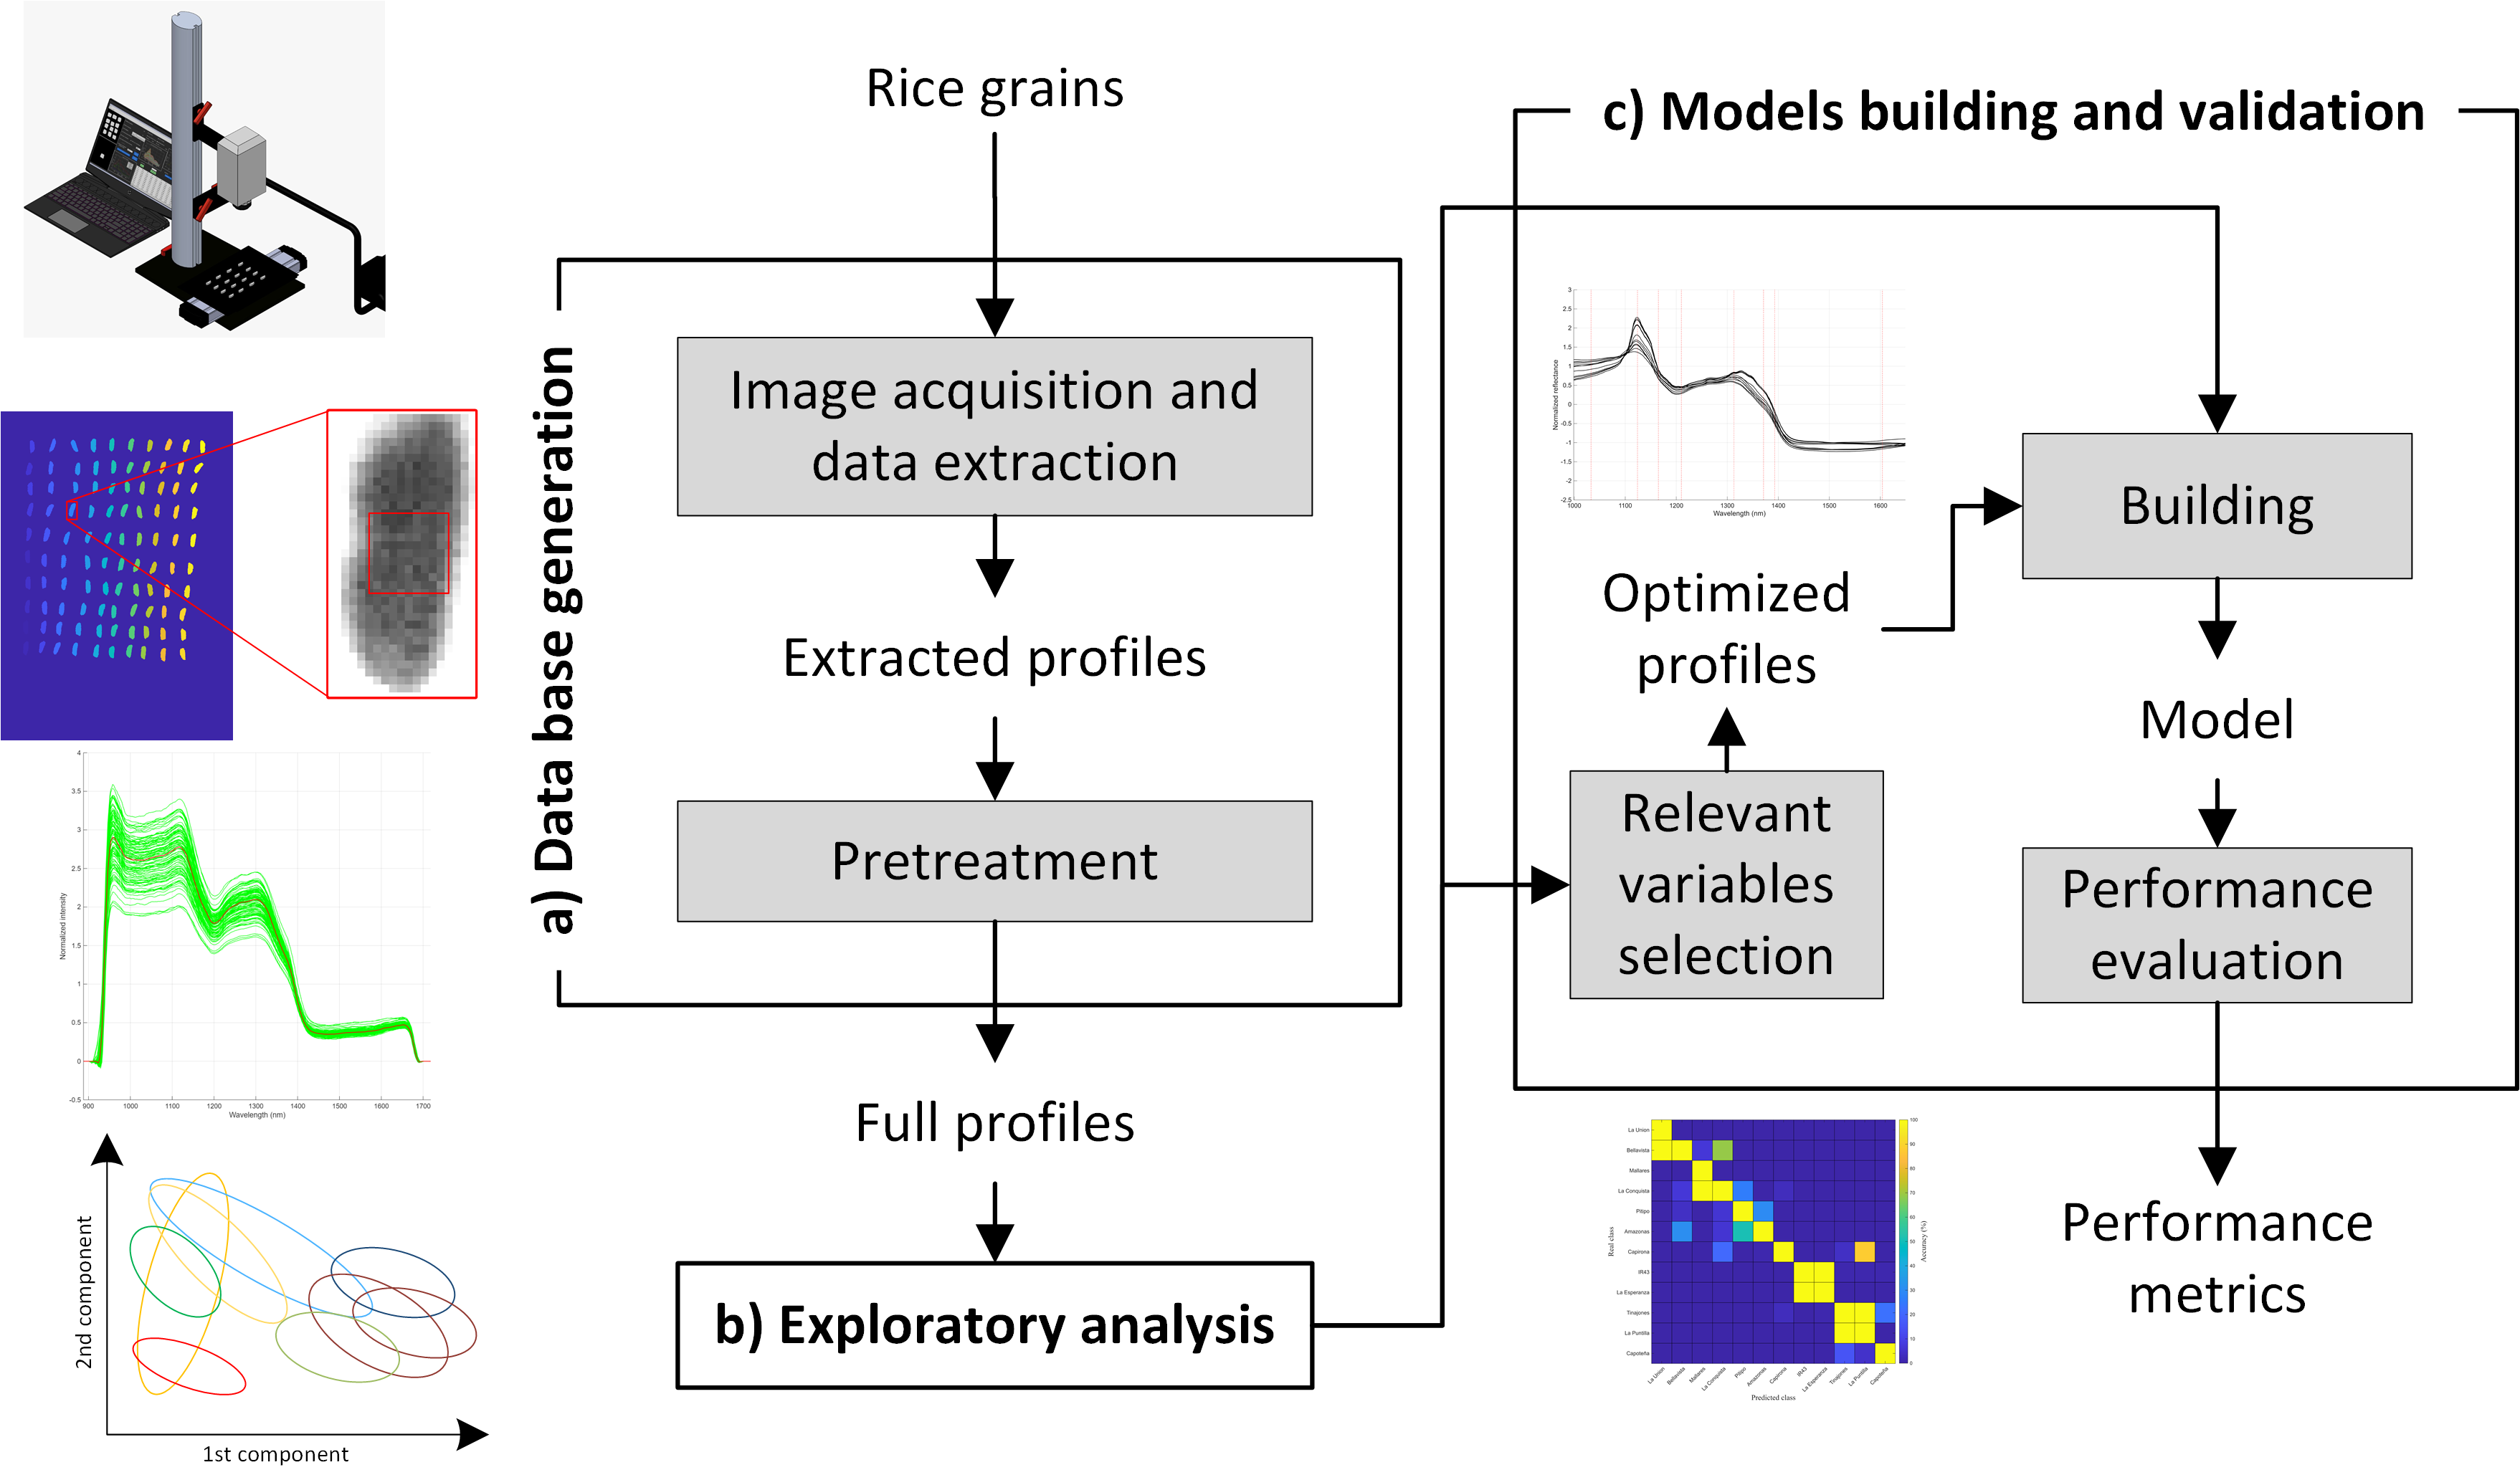
\includegraphics[width=0.9\textwidth]{Figures/Fig_01.png}
    \caption{Workflow of the methodology used in this study}
    \label{fig_01}
\end{figure*}


\subsection{Grains of rice}

% colecta de muestras

\added{Half a kilogram of each of} twelve varieties was obtained from the National Institute of Agricultural Innovation (INIA) and transported to the Food Safety Research Laboratory of the National University of Frontera (UNF); and were:  

\begin{multicols}{2}
\begin{itemize}
    \item La Unión
    \item Bellavista
    \item Mallares
    \item La Conquista
    \item Pitipo
    \item Amazonas
    \columnbreak
    \item Capirona
    \item IR43
    \item La Esperanza
    \item Tinajones
    \item La Puntilla
    \item Capoteña
\end{itemize}
\end{multicols}

The samples were stored in hermetically sealed dark bags under controlled environmental conditions (24 °C, dry environment) to maintain their spectral integrity until image acquisition.

\subsection{Database generation}\label{sec_database}

\subsubsection{Image acquisition and data extraction} 

% sobre el euipo y condiciones de toma de imagenes
Hyperspectral data were acquired using a Resonon Pika NIR-640 camera (Resonon Inc., USA) in reflectance mode \added{(336 bands, 888--1718~nm; the analysis uses the 263 contiguous bands 47--309, 999--1649~nm)}; \added{1000 grains of each rice variety were placed on a dark matte surface and imaged in blocks of 100 grains at a time.}
Acquisition was performed under controlled lighting conditions to achieve spectral stability and comparability between measurements.
\added{Finally, the data, in *.bil format, were stored on Network Attached Storage (NAS) devices for subsequent analysis.} 

% sobre la extraccion de  los perfiles
Routines and functions were implemented to visualize the information contained in the hypercubes; the intensity image at 1475 nm was used—due to the contrast difference—to segment the rice grains.
A square Region Of Interest (ROI) measuring 11 pixels per side was generated based on the center of gravity of each grain, and the mean spectral profile was extracted from it.
Finally, the mean profiles for each grain, coded by variety, were stored in an Excel spreadsheet.
\acnote{Question for UNF: the paragraph above states that 1000 grains per variety were scanned, in blocks of 100 (ten blocks per variety). The data matrix we received (\texttt{X.mat}/\texttt{Y.mat}) has only 500 spectra per variety, 6000 in total, half that number. Were only 500 of the 1000 scanned grains kept in the final matrix -- and if so, which five of the ten blocks of 100 were retained, and in what order? Or does ``1000 grains'' refer to a quantity other than the 500 rows per variety in the shared matrix (e.g. grains scanned before some were discarded on segmentation)? We need this to know the true grouping unit for the validation below. The \texttt{profile\_totales.mat} you sent on 2026-10-30 also holds 500 spectra per variety.}

\added{The 500 rows per variety of the shared matrix are taken to be five images of 100 grains in acquisition order, as described above (blocks of 100 grains); this defines the image used as the unit of grouped validation (Section~\ref{sec_building}).}


\subsubsection{Pre-treatment}

Raw hyperspectral data often contain noise due to instrumental and environmental effects \cite{vasquez2018}; therefore, a series of spectral preprocessing steps was applied, which are detailed below.

\begin{itemize}
    \item \textbf{Smoothing.} For noise reduction, the \added{Savitzky-Golay} filter was applied; this filter preserves the shape of the peaks and reduces high-frequency noise; see Equation~\ref{eq_01}.
    \begin{equation}
        y_{i,j} = \sum_{k=-m}^{m} c_{k}\, x_{i,\,j+k}
        \label{eq_01}        
    \end{equation}
    where $y_{i,j}$ is the smoothed value of the sample $i$ at the wavelength index $j$; $x_{i,\,j+k}$ is the original value of the signal; $c_{k}$ are the SG convolution coefficients determined by the degree of the polynomial $p$ and the order of the derivative $d$; $m = (w-1)/2$ is the half-width of the window; and $w$ is the total length of the window (an odd number of points), which corresponds to $w = 2m + 1$.

    \item \textbf{Normalization.} \added{The Z-score normalization method was applied to the profiles, scaling the data points} to have a mean $(\mu)$ of 0 and a standard deviation ($\sigma$) of 1, see Equation~\ref{eq_02}.
    \begin{equation}
        X_{Norm} = \frac{X-\mu}{\sigma}
        \label{eq_02}
    \end{equation}
    \added{where} $X_{Norm}$ \added{is} the normalized profile with Z-score, X is the raw profile, $\mu$ mean, and $\sigma$ the standard deviation of the profile.
\end{itemize}

\subsection{Exploratory analysis}

\added{As in} \citet{amigo2013,zhang2022,ali2024}\added{,} the principal component analysis was performed using the \emph{pca} function provided by MATLAB \added{on} the standardized data matrix.
The projection of the observations onto the first two principal components was visualized through a scatter plot, using distinct colors and markers per class, with confidence ellipses superimposed to assess dispersion and overlap between groups. 

\subsection{Model building and validation}

The modeling step was designed to systematically compare different supervised classification strategies, identify the most informative spectral variables, and optimize previously implemented models using relevant variables. 
The pipeline comprised three complementary stages: 
\begin{itemize}
    \item [i] Construction and training of the classification models, 
    \item [ii] Selection of relevant variables using three alternative feature-selection approaches 
    \item [iii] Evaluation of classification performance through averaged confusion matrices and quantitative metrics per-class. 
\end{itemize}

For each step, the functions shared the same predictor matrix X, class vector Y, and  spectral band vector Z, ensuring full reproducibility and direct comparability of the results across configurations.


\subsubsection{Building}\label{sec_building}

The construction of the classifiers was carried out through \added{a five-fold cross-validation repeated six times (30 splits); the original MATLAB analysis used a 70/30 hold-out repeated 30 times.}
\added{Each split tests 20\% of the grains of each variety and every grain is tested six times. Two versions of the division were compared. In the \emph{random} version, individual grains were assigned to folds at random within each variety, as is usual in the field. In the \emph{grouped} version, whole images of 100 grains were assigned to folds, so that each split holds out one image per variety and grains imaged together never appear on both sides. The random version estimates accuracy on grains from images already seen during training; the grouped version estimates accuracy on grains from another image, which is closer to how an instrument would be used.}

\begin{itemize}
    \item [a] Linear Discriminant Analysis (LDA).
    This model, see Figure~\ref{fig_models}a, seeks a linear combination of variables that provides discrimination between classes \cite{Rahmani2022}.
    \added{It was fitted as a single multiclass model with a pooled covariance matrix (scikit-learn \texttt{LinearDiscriminantAnalysis}, the equivalent of MATLAB \texttt{fitcdiscr}). The original MATLAB analysis used \texttt{templateLinear}, which builds a linear SVM learner rather than an LDA, with a solver that stopped before convergence; that model is kept under its proper name, L-SVM (item b), alongside this true LDA.}
    \item [\added{b}] \added{Linear SVM with a linear-learner template (L-SVM). This is MATLAB's \texttt{fitcecoc} with a \texttt{templateLinear} learner and its defaults: one-vs-one binary linear SVMs with hinge loss and ridge penalty $\lambda=1/n$, fitted on the bands without standardisation. It is fitted to convergence; it differs from the SVM below mainly in the absence of standardisation.}
    \acnote{Item [b] is the model labelled LDA in your analysis (\texttt{fitcecoc} + \texttt{templateLinear}), now under its proper name; the true LDA is item [a]. With its defaults (SVM learner, ridge, $\lambda=1/n$, dual solver, no standardisation) it gives 90.2\% when fitted to convergence and 71.2\% when stopped after about 20 passes, which reproduces the 71.7\% implied by your Table~3. Python equivalents of all four models are now in the text (Section~2, first paragraph). Scripts \texttt{10\_Validacion\_UNF.py} and \texttt{13\_Tabla3\_recalculada.py}.}
    \item [\added{c}] Support Vector Machine (SVM).
    This model constructs an optimal separation hyperplane between classes and the decision boundary which is determined by maximizing the margin between the hyperplane and the closest samples, known as support vectors (Figure~\ref{fig_models}b). 
    \added{In addition,} kernel functions can be used to address nonlinear classification problems \cite{Onmarkhong2022, castro2019}.
    A multiclass SVM with a linear kernel and standardized predictors was implemented through an Error-Correcting Output Codes (ECOC) scheme (fitcecoc with templateSVM('Standardize', true)).
    \item [\added{d}] Artificial Neural Network (ANN).
    In this case, interconnected processing units, called neurons, are organized into layers and learn nonlinear relationships between input variables and outputs by adjusting connection weights. 
    In the specific case of the neural network of backpropagation, learning involves forward propagation of information followed by backward propagation of the prediction error to update the network parameters (Figure~\ref{fig_models}c) \cite{Kang2024, castro2019}.
    A feed-forward network with a single hidden layer was trained via fitcnet with standardized inputs ('Standardize', true) and a hidden layer of \added{$\sqrt{p}$} neurons, where $p$ denotes the number of predictors.
    \acnote{The September text said ``square of p''; Figure~\ref{fig_models}c of your October version gives $\sqrt{p}$ neurons (about 16 for the full spectrum), so we corrected the text and withdrew our earlier note about a $p^2$ layer. Our Python replication also used 16 hidden units.}
\end{itemize}

\begin{figure}[htbp!]
    \centering
    \subfloat[]{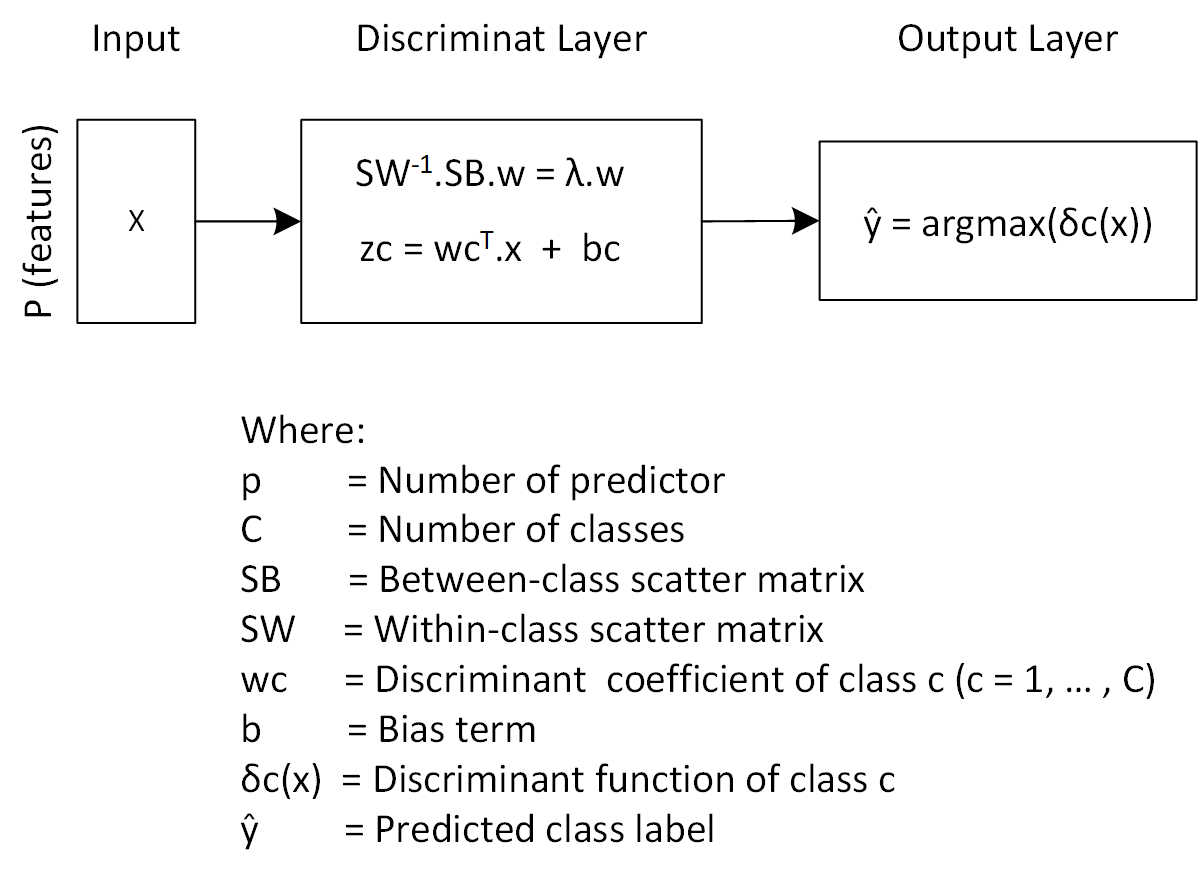
\includegraphics[width=0.85\columnwidth]{Figures/model_LDA.png}}\\ 
    \subfloat[]{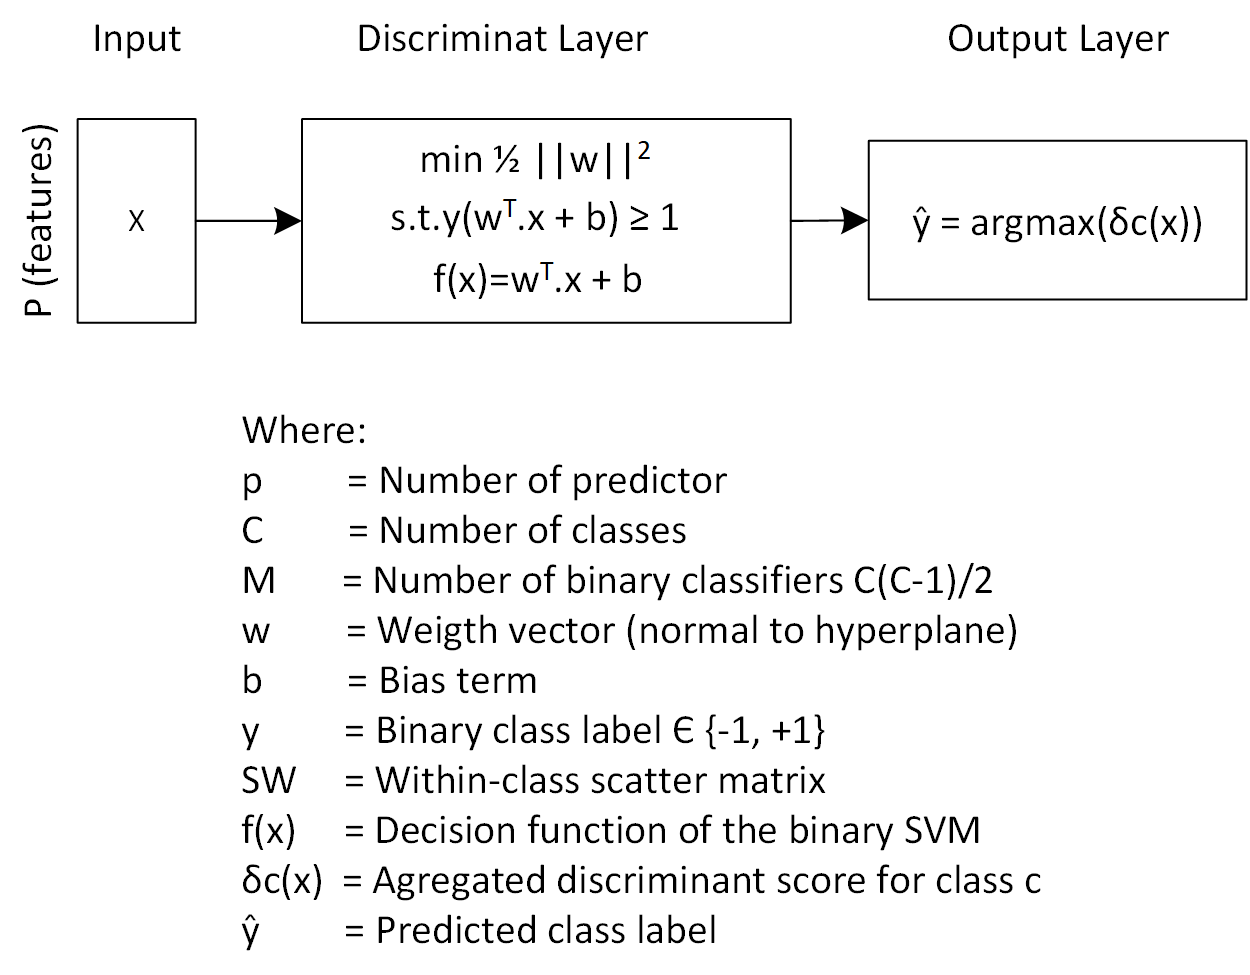
\includegraphics[width=0.85\columnwidth]{Figures/model_SVM.png}}\\
    \subfloat[]{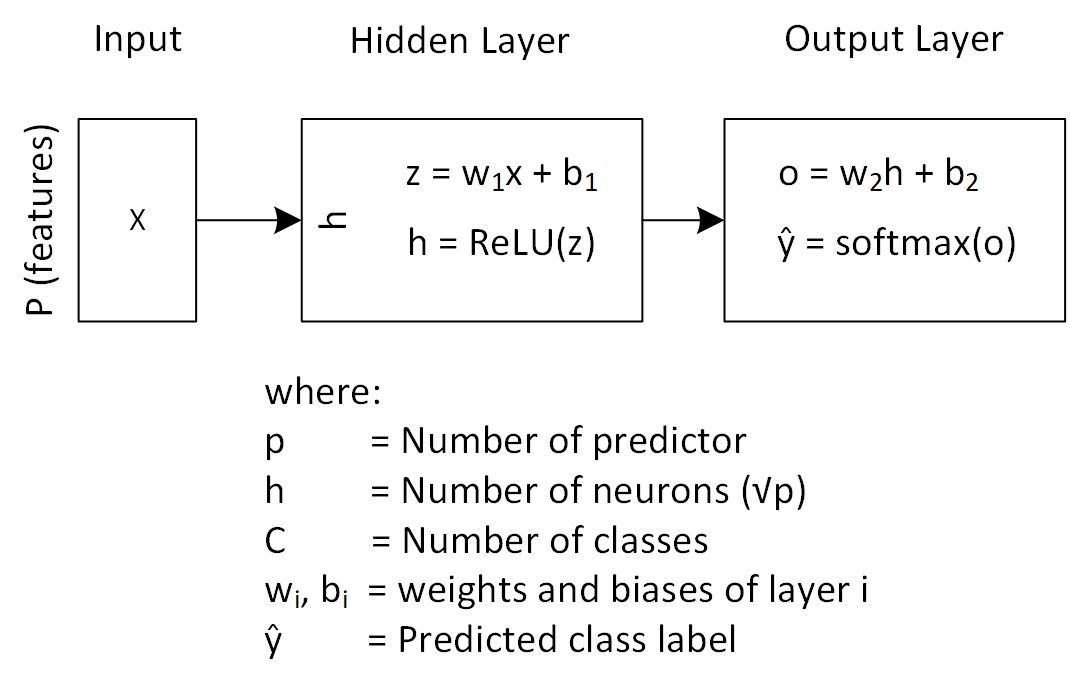
\includegraphics[width=0.85\columnwidth]{Figures/model_ANN.png}} 
    \caption{Schematic diagram for models a) LDA, b) SVM, and c) ANN}
    \label{fig_models}
\end{figure}


\subsubsection{Selection of relevant variables}\label{sec_feature_selection}

Three alternative feature selection strategies were implemented to identify the most relevant spectral bands and to compare their effect on classification performance \cite{Rahmani2022, Castro2022cafs}: 

\begin{itemize}
    \item [-] Feature Selection by Neighborhood Component Analysis (FSCNCA).
    This supervised method assigns a weight to each feature based on its contribution to prediction. 
    Features with larger weights are considered to be more relevant, whereas features with small weights can be removed to obtain a reduced representation of the original feature space.
    The implementation applies the fscnca function with a stochastic gradient descent solver ('Solver','sgd') to estimate a relevance weight for each spectral band. 
    To determine an appropriate cut-off threshold, the function was evaluated in a range of candidate thresholds (from \added{1} to 6 in steps of 0.5) and, for each threshold, the number of variables was calculated to obtain a similar number of variables than for the other methods. \added{In the reported run the sweep was not used: a fixed threshold of 3.6 was applied, which retained nine bands.}
    \acnote{In the threshold sweep of \texttt{Sel2VarFSCNCA}, the SVM inside the loop is trained on the full \texttt{X}, not on \texttt{X(:,pos)}, so every threshold returns the same score and the sweep does not compare thresholds. In the run reported the sweep was switched off (\texttt{LimRec = [1, 3.6]}) and the threshold fixed at 3.6, which is what we state above.}
    
    \item [-] Sequential Forward Selection (SFS).
    This is a wrapper-based method that starts with an empty feature subset and sequentially adds the feature that produces the greatest improvement according to a predefined model-performance criterion.
    The process progressively constructs a reduced feature subset without exhaustively evaluating all possible combinations. 
    The implementation uses an LDA classifier as the evaluation criterion, starting from an empty feature set; iteratively evaluating all remaining candidate features and selecting, at each step, the one that maximizes the mean 5-fold cross-validated accuracy (cvpartition(Y,'KFold',5)). 
    The procedure continues for a maximum of \added{$k=9$} iterations and stores the estimated accuracy at each step in the vector accuracy; if no feature is selected (e.g., due to classification failures), the function is relegated to selecting the variable with the highest variance. 

    \item [-] Covering Array Feature Selection (CAFS).
    It is a supervised wrapper approach based on covering arrays, combinatorial structures characterized by high interaction coverage with a reduced number of configurations. 
    CAFS uses the subset of experiments defined by the covering array to explore the feature space and identify the features that maximize a predictive-performance criterion, such as the F1 score.
    This enables the exploration of relevant feature interactions with substantially fewer combinations than an exhaustive search.
    The implementation is based on previously reported work by \citet{Castro2022cafs}, and uses a Naive Bayes classifier ('nb') \added{within a nested cross-validation: 5 outer folds, 5 inner folds to score the candidate subsets, and 3 folds to optimise the hyperparameters of the classifier}.
    \acnote{The draft cited this method to an unrelated, unidentifiable "Avila (2024)" work. Covering Array Feature Selection (CAFS) paired with a naive Bayes classifier was introduced by Castro, De-la-Torre, Avila-George, Torres-Jimenez, Guivin and Acevedo-Ju\'arez (2022), \emph{Spectrochimica Acta Part A}, vol.~270, art.~120815, DOI~10.1016/j.saa.2021.120815 -- note that Wilson Castro, a co-author of this manuscript, is the first author of that paper, and Himer Avila-George is a co-author, not the lead author; neither the year nor the attribution in the original placeholder was correct. A 2024 follow-up by Tirado-Kulieva, Quijano-Jara, Avila-George and Castro applies CAFS to coffee fermentation, but that study optimises a PLSR model, not a naive Bayes classifier, so it is not the source of the method described here. The citation above has been corrected accordingly.}
    The algorithm was configured with the following options: 
    \begin{itemize}
        \item Patience parameter (Patience = 3)
        \item Minimum improvement threshold (MinImprovement = 1e-4)
        \item Minimum number of features (MinFeatures = 10)\added{; the subset is halved until it has no more than this number of bands, so the subset returned can be smaller}
        \item Maximum number of iterations (MaxIterations = 50)
        \item Random seed (RandomSeed = 42)
        \item \added{Target number of features (TargetFeatures = 20)}
        \item \added{Compactness penalty (CompactnessPenalty = 0.10, ExcessPenaltyPower = 2, AdaptivePenaltyAlpha = 2)}
    \end{itemize}

     Spectral preprocessing was also applied using standard normal \added{variate} (SNV) to reduce multiplicative scattering and baseline differences between samples, and a target-excess compactness penalty was included that discourages the selection of subsets larger than the target number of wavelengths. 
     \added{The five outer folds selected between 9 and 25 bands, with an outer accuracy of the naive Bayes classifier of $71.6\pm2.1$\%; only the band at 1012~nm was chosen in all five folds. The subset carried forward to the classifiers of Section~\ref{sec_building} is the one of the first outer fold: nine bands at 1012, 1063, 1232, 1234, 1420, 1435, 1624, 1639 and 1649~nm.}
        
\end{itemize}

\added{\textbf{Random-subset baseline.} Because neighbouring NIR bands are strongly correlated, a small set of bands drawn at random may already carry most of the discriminant information. To judge whether a selection method identifies informative bands, rather than merely reducing their number, each selected subset was compared against 30 subsets of the same size drawn uniformly at random from the 263 bands and evaluated with one image per variety held out. The nine-band subsets of the original MATLAB analysis were compared in the same way with 30 random nine-band subsets on each of the 30 splits of Table~\ref{tab:acc}, with one image per variety held out. Selection itself was evaluated on ten splits (two repetitions of the grouped five-fold cross-validation with one image per variety held out). In this baseline, unlike in the MATLAB analysis described next, selection was fitted on the training part of each split only, so that the test grains take no part in choosing the bands.}
\added{In the original MATLAB analysis each selection method was applied once, before the hold-out repetitions: FSCNCA and SFS on all 6000 spectra, and CAFS on the training part of its first outer fold (80\% of the spectra), so the test grains took part in choosing the bands. Here, as stated above, selection is fitted on the training part of each split only.}
\acnote{Confirmed by your script (received 2026-10-30), so it is now stated in the text. The fix is to run each selection inside the training part of every repetition, as in our baseline (Section~\ref{sec_bands_results}).}

\subsubsection{Performance evaluation}\label{sec_performance}

The classification performance was evaluated through two complementary procedures: 

\begin{itemize}
    \item [-] Generation of average confusion matrices. 
    For each repetition, a confusion matrix is computed using confusionmat, and the resulting matrices are averaged across the N iterations to obtain a representative confusion matrix. 
    Each row of this averaged matrix is then normalized to percentages, yielding a row-wise accuracy representation that facilitates the interpretation of \added{per-class performance} independently of class size and displayed as a heatmap.
   
    \item [-] Calculation of quantitative \added{per-class} metrics. For each iteration, the following quantities were derived from the confusion matrix: true positives (TP, diagonal elements), false positives (FP, column sums minus TP), false negatives (FN, row sums minus TP), and true negatives (TN, total minus (FP + FN + TP)). 
    From these, \added{three} standard metrics were calculated per class and per iteration: precision, defined as TP / (TP + FP); recall (sensitivity), defined as TP / (TP + FN); and the F1-score, defined as the harmonic mean 2·(Precision·Recall) / (Precision + Recall).
    The structure of the confusion matrix and these ratios are shown in Figure~\ref{figCM}, and the metrics were calculated in a way similar to \citet{castro2019}, see Equations~\ref{eq_acc} to \ref{eq_fm}\added{; Equation~\ref{eq_acc} is the overall accuracy over all classes, and Equations~\ref{eq_pre}--\ref{eq_fm} are per class}.

    \begin{figure}[htbp!]
        \centering
        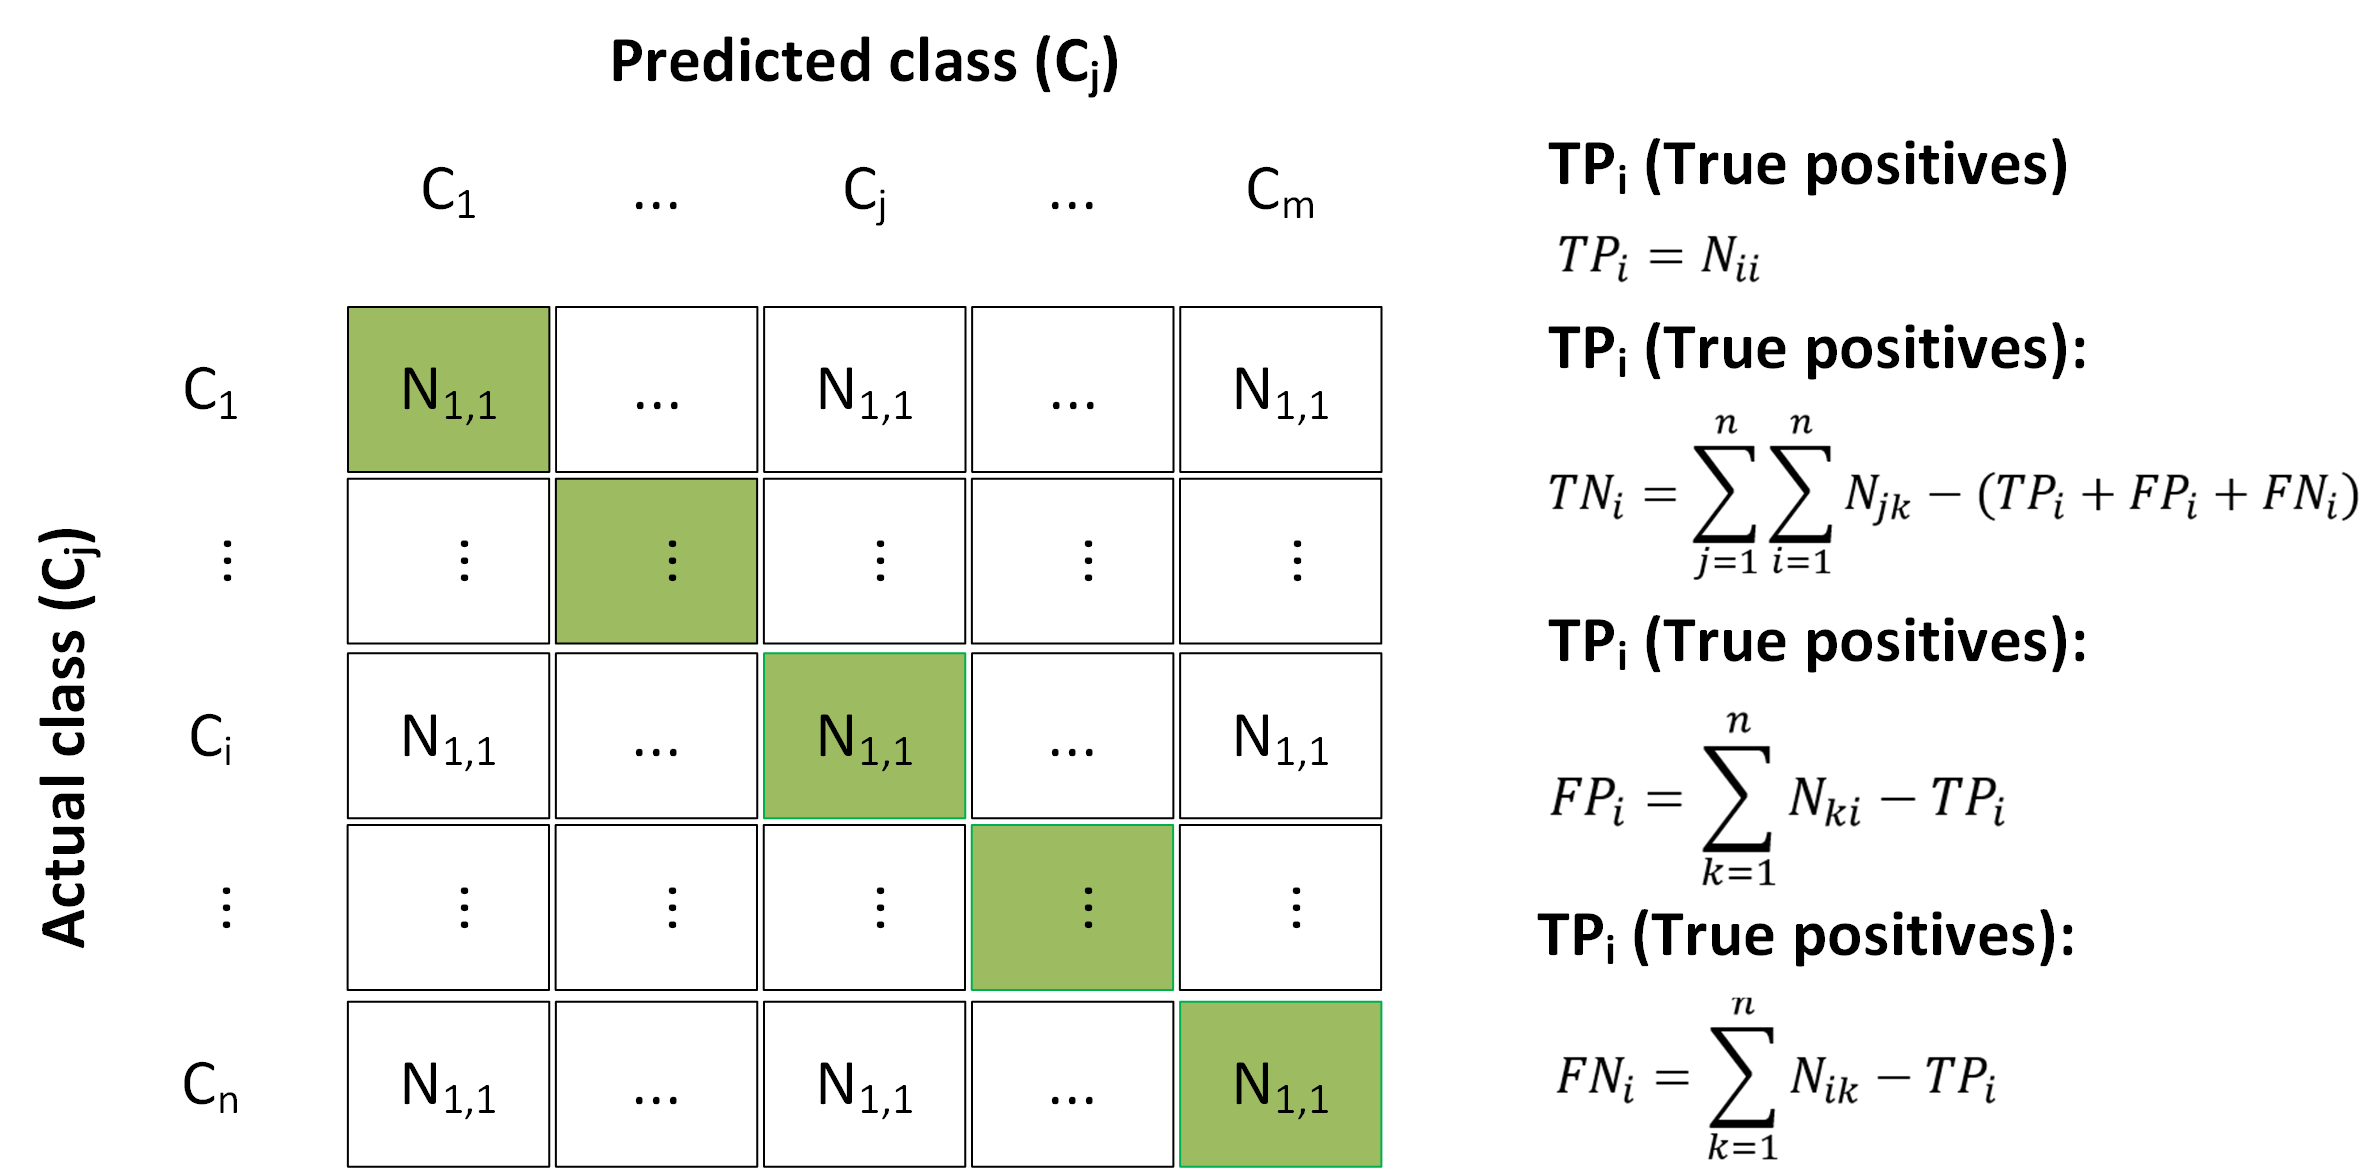
\includegraphics[width=1.0\columnwidth]{Figures/fig_CM.png}
        \caption{CM structure and main ratios}
        \label{figCM}
    \end{figure}

    \begin{equation}
        Accuracy \, (acc) = \frac{\sum_{i=1}^{K}TP_{i}}{\sum_{i=1}^{K} \sum_{j=1}^{K}N_{ij}}
        \label{eq_acc}
    \end{equation}
    \begin{equation}
        Precision \, (pre) = \frac{TP_{i}}{TP_{i} + FP_{i}}
        \label{eq_pre}
    \end{equation}
    \begin{equation}
        Recall \, (rec) =  \frac{TP_{i}}{TP_{i} + FN_{i}}
        \label{eq_rec}
    \end{equation}
    \begin{equation}
        F\text{-}measure_{i} \, (FM) =  2\left(\frac{pre_{i}\cdot rec_{i}}{pre_{i}+rec_{i}}\right)
        \label{eq_fm}
    \end{equation}
    \acnote{Table~\ref{tab:acc} now reports overall accuracy (Equation~\ref{eq_acc}), recomputed by us with your protocol; the per-class one-vs-rest values computed by your \texttt{metricas\_CMH} are no longer used. We also relabelled the F-measure equation, which shared the label of the recall equation.}
\added{Overall accuracy was defined as the proportion of test grains assigned to their correct variety, $\sum_c \mathrm{TP}_c / N$, and summarised together with the macro-averaged F1-score. The per-class one-vs-rest accuracy $(\mathrm{TP}+\mathrm{TN})/N$ was not used as a summary: with $K$ classes and overall error $e$, its mean over classes equals $1-2e/K$ exactly, whatever the class balance, because every misclassified grain counts once as a false negative and once as a false positive. It therefore carries no information beyond overall accuracy, compresses differences by a factor $K/2$, and cannot fall below $1-2/K$: for $K=12$ an overall accuracy of 97\% appears as 99.5\%, random guessing scores 84.7\%, and a classifier that is always wrong still scores 83.3\%.}
    For each metric, the mean and standard deviation over the \added{30 splits} were calculated; this procedure was repeated for each classifier and each feature configuration considered in the study (full profile and the three optimized subsets obtained in Section~\added{\ref{sec_feature_selection}}), allowing a systematic comparison of predictive performance between models and feature subsets and providing the empirical basis for selecting the most suitable combination of classifier and feature representation.
    \acnote{Question for UNF: was any statistical criterion (e.g.\ a significance test) used to decide whether two configurations -- two classifiers, a selection method against another, or a selection method against the random-subset baseline of Section~\ref{sec_feature_selection} -- give meaningfully different accuracy? Or were conclusions drawn by comparing the reported means and standard deviations directly, without a formal test?}
    \added{We applied an explicit criterion to our analysis (Sections~\ref{sec_classification} and \ref{sec_bands_results}). The 30 splits reuse the same 60 images, so they are not independent observations and tests on them overstate the evidence \citep{Nadeau2003}. Classifiers were therefore compared at the level of images: the accuracy of each image was averaged over the repetitions in which it was tested, the classifiers were compared in pairs over the 60 images with the Wilcoxon signed-rank test, and 95\% confidence intervals for the differences were obtained by resampling images (10\,000 bootstrap samples); random and grouped division were compared in the same way, paired by image. Band subsets were compared with random subsets on each split (paired $t$-test and Wilcoxon test over the splits); these comparisons share the same limitation, so their $p$-values indicate how consistent a difference is across splits rather than giving formal evidence. $P$-values were adjusted with the Holm procedure within each family (12 classifier comparisons; 4 drops from random to grouped division; 12 comparisons of the original nine-band subsets with random subsets; 30 comparisons of training-only selections with random subsets), and a difference is reported as significant at an adjusted $p<0.05$.}

\end{itemize}



% ================================================================================================
%% RESULTS AND DISCUSSIONS
% ================================================================================================

\section{Results}

\subsection{Mean profiles}\label{sec_mean_profiles}

\begin{figure}[htbp!]
    \centering
    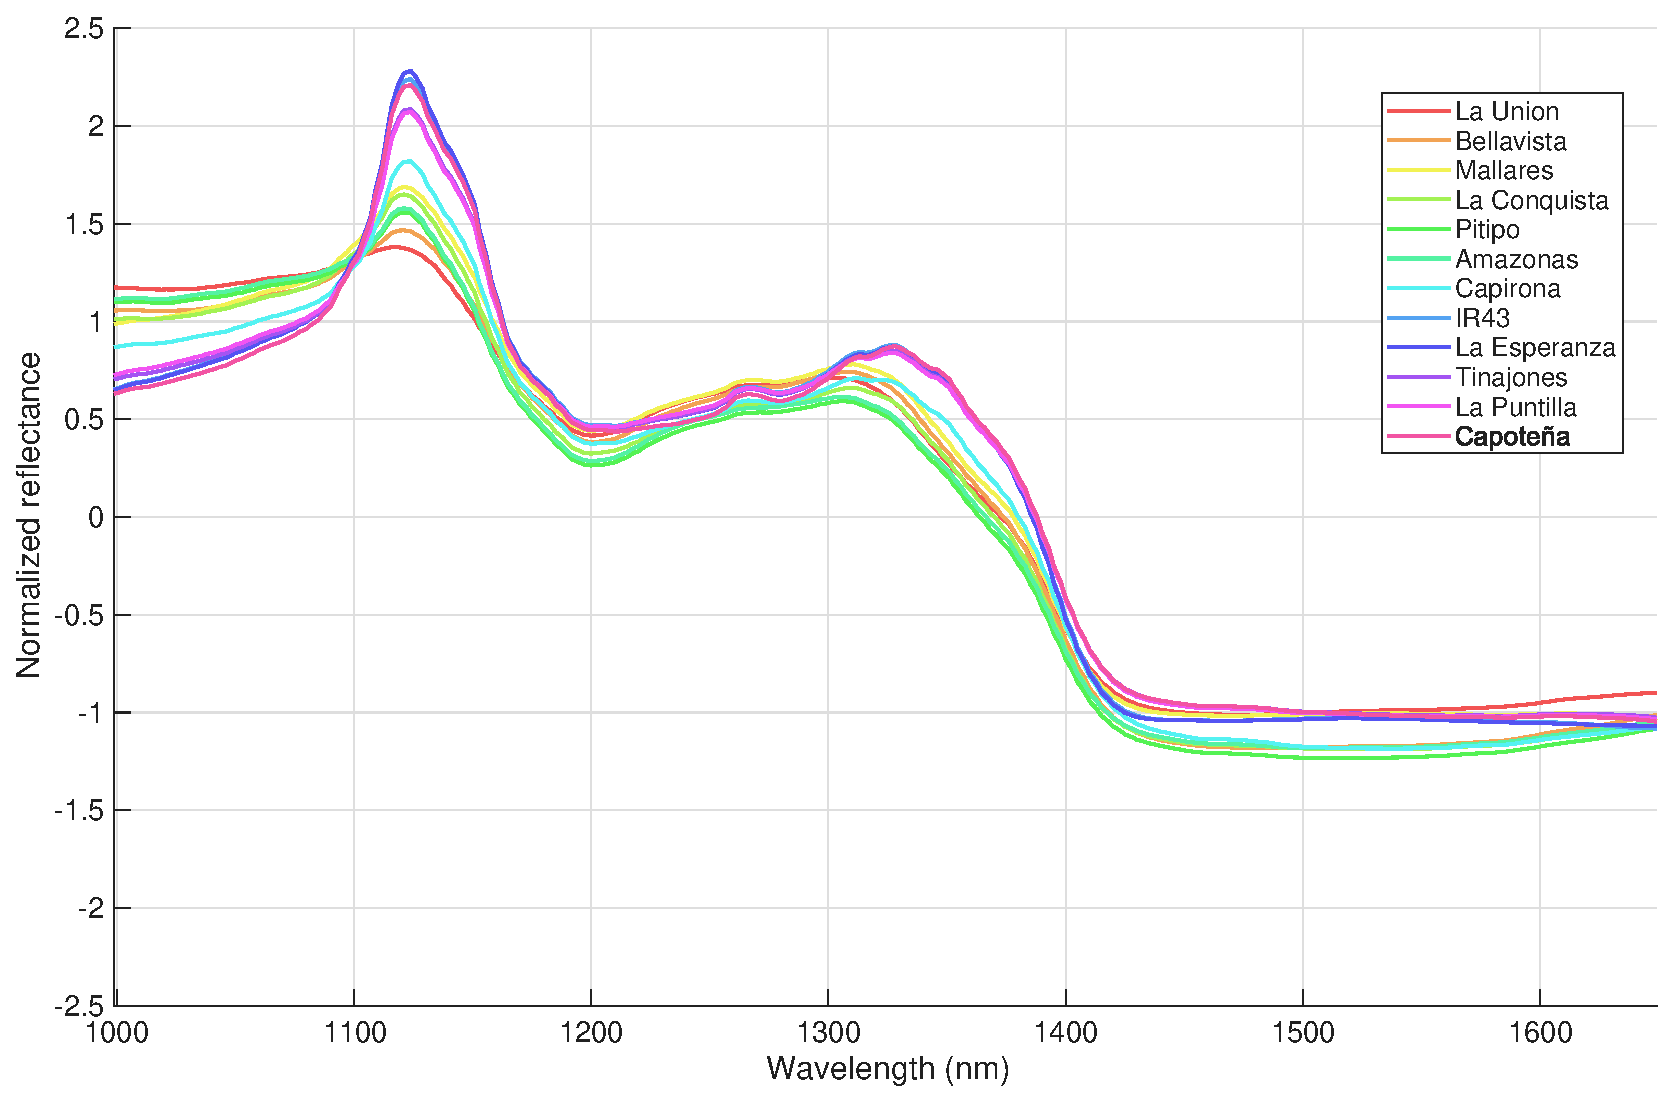
\includegraphics[width=\columnwidth]{Figures/Fig_prof_means.eps}
    \caption{Mean profiles of each variety}
    \label{fig_02}
\end{figure}

\added{Figure~\ref{fig_02} shows the mean profile of each variety after Savitzky-Golay smoothing and Z-score normalisation. The profiles are reflectance, so absorption bands appear as minima and as the falling edges that lead into them, while maxima are windows of comparatively weak absorption between bands. All twelve profiles share the same shape: a rising edge from 1000~nm to a reflectance maximum near 1120--1125~nm, a sharp fall to a minimum near 1195--1200~nm, a secondary maximum near 1300--1330~nm, a steep fall between about 1340 and 1430~nm, and a low, nearly flat plateau from 1430~nm to the end of the range near 1650~nm, where the varieties differ little. Varieties differ mainly in amplitude rather than in position: the highest maxima near 1120 and 1300~nm belong to the same two or three varieties throughout, and the lowest to a different, consistent subset. In this range the varietal signal is therefore carried by the depth of the absorption features and the height of the windows between them, not by shifts in wavelength.}
\added{The minimum near 1195--1200~nm lies in the second-overtone region of C--H stretching of CH$_2$ and CH$_3$ groups \citep{Workman2012}. On rice grain, \citet{John2022nirs}, surveying 500 brown rice accessions, assign 1196~nm to ``the C--H second overtone corresponding to aliphatic hydrocarbons'', and \citet{Onmarkhong2022} assign 1202~nm to the second overtone of the symmetric C--H stretching of CH$_3$ groups, associated with amylose. The falling edge that leads into this minimum, from the maximum near 1125~nm, covers the band that \citet{Shao2011starch} found in second-derivative absorbance spectra of rice flour at 1131--1155~nm and assigned to C--H stretching of starch (they call it the first overtone; standard tables place C--H second overtones in this region \citep{Workman2012}). The C--H absorption near 1200~nm thus combines starch and lipid, and the single band does not by itself separate the two. The fall between 1340 and 1430~nm and the low plateau beyond it are the first-overtone O--H absorption of water, which \citet{Shao2011starch} place at 1418~nm in rice flour, together with C--H combination bands near 1360--1420~nm \citep{Workman2012}; the plateau also spans the first overtone of N--H stretching of protein near 1500--1530~nm and the O--H stretching of starch near 1580~nm \citep{Onmarkhong2022}. The maxima near 1120 and 1300~nm are not absorption bands: their height reflects how deep the neighbouring bands are and how strongly the grain scatters. Band positions shift with the matrix, so we rely on the rice studies \citep{Shao2011starch,John2022nirs,Onmarkhong2022} for specific positions and use the general tables only at the level of spectral regions.}
The broad characteristic between approximately 1250 and 1340 nm should be interpreted as an overlapping response of the rice matrix rather than being assigned to a single constituent.
The pronounced decrease in reflectance around 1400–1450 nm corresponds to the first overtone of OH stretching and has been associated with the OH groups of water, starch and amylose in rice \cite{Onmarkhong2022}.
At longer wavelengths, the characteristic around 1580 nm has been associated with O-H stretching involving intermolecular hydrogen bonding in starch and glucose \cite{Onmarkhong2022}.
Therefore, the spectral differences between the twelve varieties are mainly consistent with variations in starch matrix, amylose-related composition, moisture, and molecular interactions.
\acnote{Rewritten after an external review (2026-10-30): the profiles are reflectance (your MATLAB plots label them ``Normalized reflectance''), so absorption bands are the minima. The previous text read the maxima near 1120 and 1300~nm as starch absorption peaks, which inverts the sign; the assignments now sit on the minimum near 1200~nm and on the falls into the O--H region. Your 1202~nm CH$_3$ assignment \citep{Onmarkhong2022} is now placed at that minimum, where it is sign-consistent. The general tables for pasture and \emph{Eucalyptus} were replaced by a standard compilation \citep{Workman2012}, and the closing sentence citing CAFS for the compositional relevance of wavebands was removed, since it does not bear on rice.}

\subsection{Exploratory analysis}

\begin{figure}[htbp!]
    \centering
    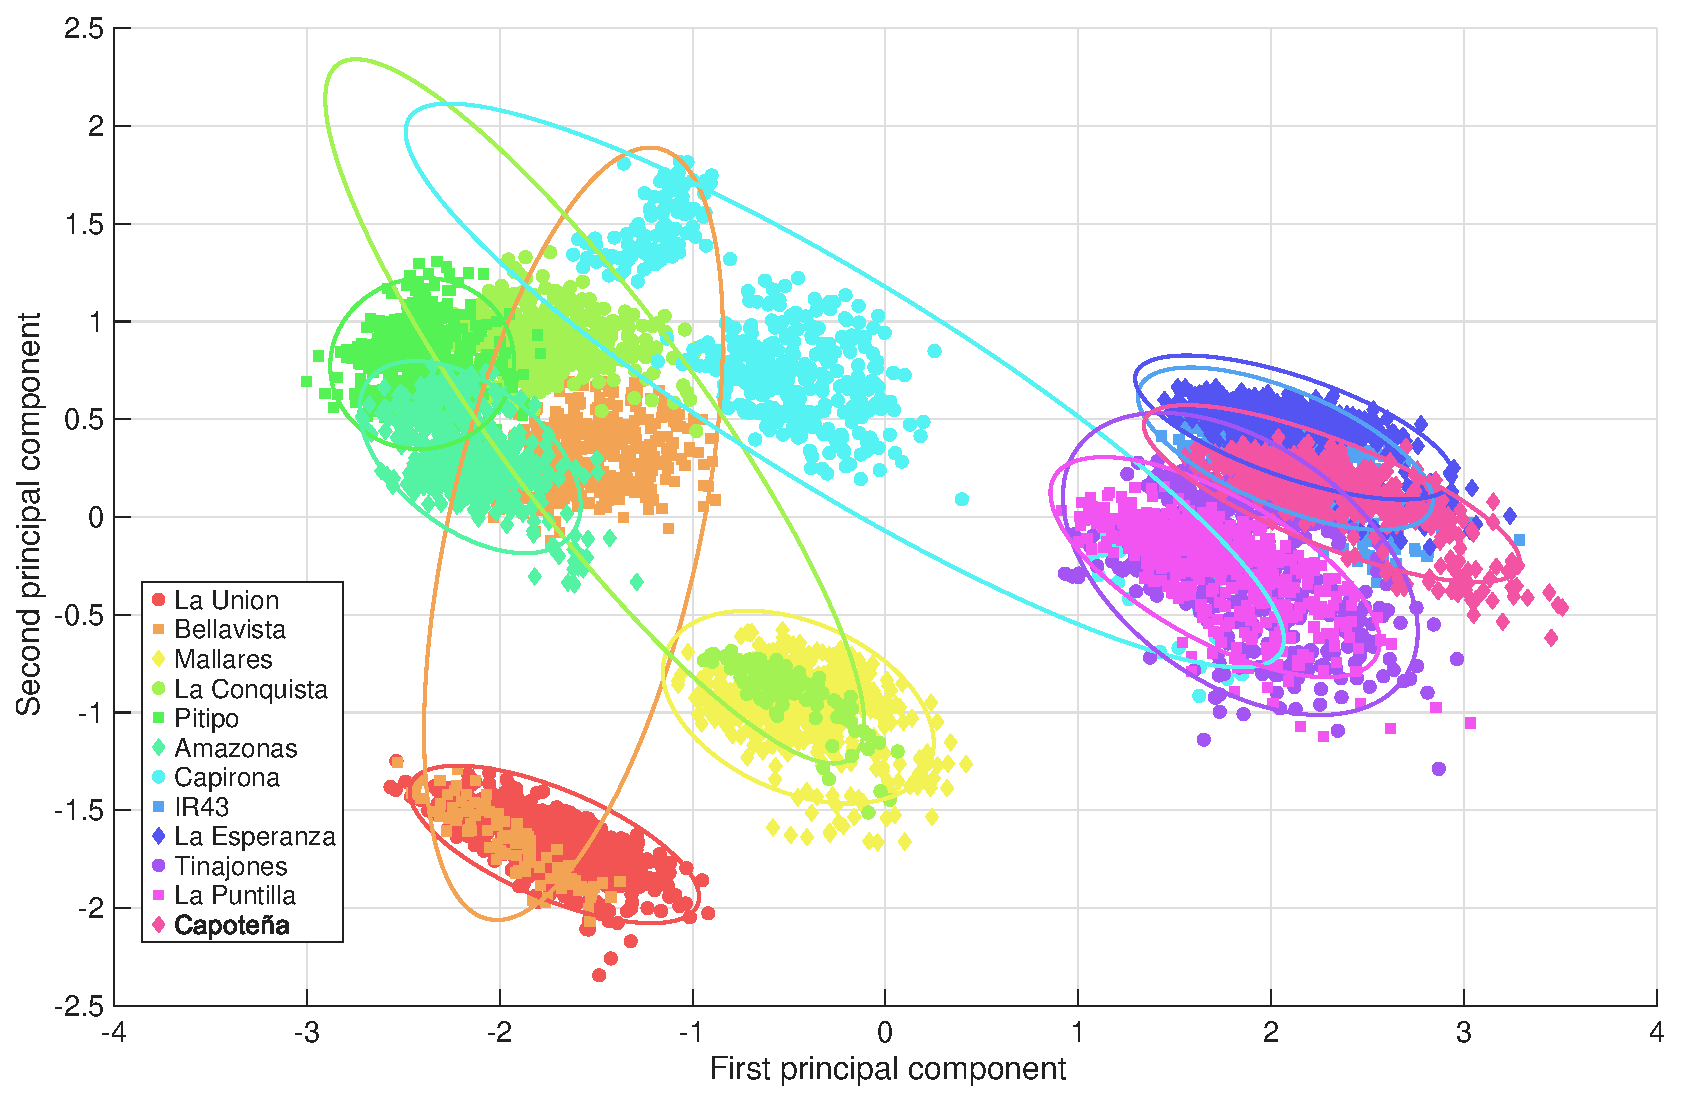
\includegraphics[width=\columnwidth]{Figures/Fig_PCA.eps}
    \caption{PCA for spectral profiles}
    \label{fig_03}
\end{figure}

Figure~\ref{fig_03} shows the PCA score plot obtained from the NIR spectral profiles of the twelve rice varieties. 
PCA transforms highly correlated spectral variables into a reduced set of orthogonal components that capture the main sources of spectral variability. 
Consequently, samples with similar NIR profiles are projected close to each other, whereas differences in spectral shape and intensity lead to separation in the PCA space. 
This behavior has been demonstrated for rice using FT-NIR spectroscopy, where PCA revealed spectral patterns associated with varietal and geographical differences \cite{Tong2021}. 
Thus, PCA summarizes the combined variations across the NIR spectrum rather than separating samples according to a single wavelength or chemical compound\added{;} similar studies using vibrational spectroscopy and PCA have shown that multivariate spectral fingerprints can reveal natural groupings and support subsequent classification or discrimination \cite{Giang2020b, Castro2022cafs}.

\added{Figure~\ref{fig_03} projects the spectra onto the first two principal components, with a 95\% confidence ellipse per variety. The first component separates two broad groups: seven varieties at negative scores (La Uni\'on, Bellavista, Mallares, La Conquista, Pitipo, Amazonas, Capirona) and five at positive scores (IR43, La Esperanza, Tinajones, La Puntilla, Capote\~na). Within the second group the second component partly separates IR43, La Esperanza and Capote\~na (upper) from Tinajones and La Puntilla (lower), with heavy overlap inside each pair. Within the first group, La Uni\'on forms a compact cloud at the bottom, Mallares a distinct cloud at the centre, and Pitipo and Amazonas overlap at the upper left. Three varieties -- Bellavista, La Conquista and Capirona -- each appear as two separate clouds rather than one: part of Bellavista lies with La Uni\'on and part near Amazonas, part of La Conquista near Pitipo and part with Mallares, and Capirona in two lobes at the upper centre. This splitting is what stretches their ellipses across the plot; these three varieties are the ones with an image classified almost entirely as another variety (Section~\ref{sec_limitations}). The first two principal components therefore group the twelve varieties into three or four blocks rather than resolving them individually, consistent with the classifiers' reliance on many discriminant dimensions (Section~\ref{sec_building}) rather than on a simple two-dimensional separation.}
\added{In a principal component analysis of the mean-centred matrix (263 channels), the first component alone carries 77.6\% of the total variance, the first two together 92.4\%, five components are needed to reach 99.4\%, and eleven for 99.9\%. The limited class separation visible here is therefore a two-dimensional cut through a signal that needs far more than two components to be summarised adequately, which is consistent with the classifiers using many discriminant or SVM dimensions rather than two.}

\subsection{Feature selection}

\begin{figure*}[htbp!]
    \centering
    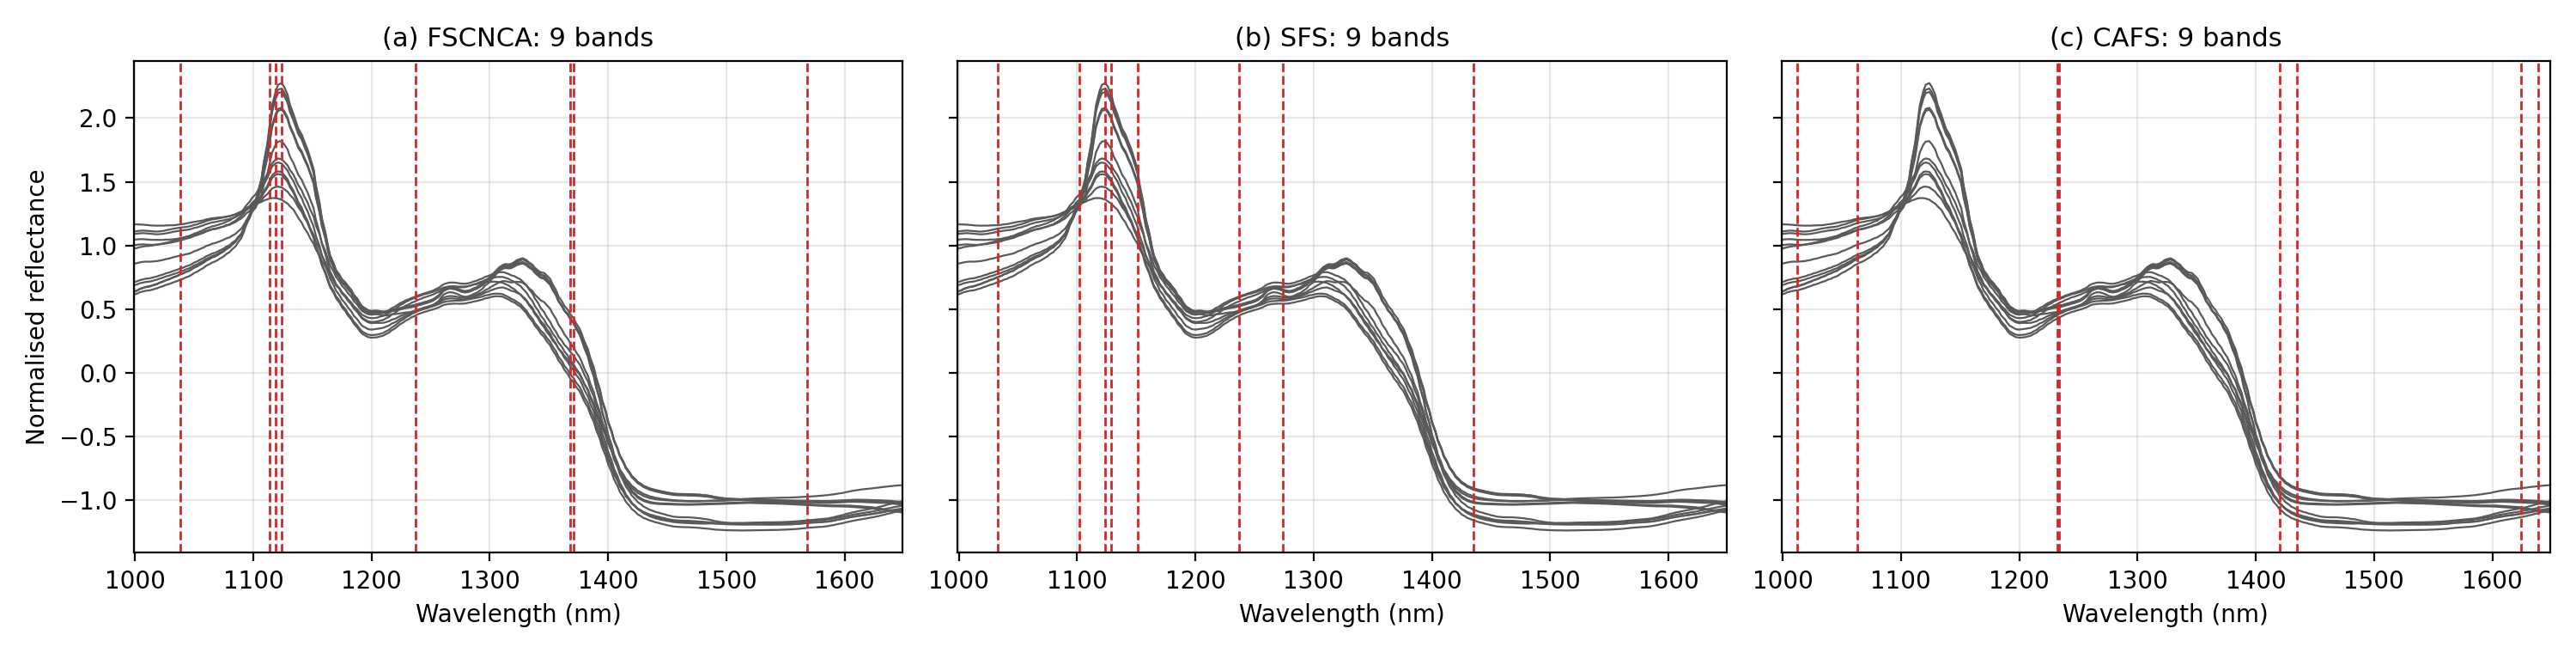
\includegraphics[width=\textwidth]{Figures/fig_unf_bandas_matlab.png}
    \caption{Relevant features using \added{a) FSCNCA, b) SFS, c)} CAFS\added{: the nine bands selected by each method in the MATLAB analysis (red dashed lines) on the mean reflectance profiles of the twelve varieties. Redrawn from the exact band positions of the original figures.}}
    \label{fig_04}
\end{figure*}

\acnote{The submitted figures and tables spell these three method names inconsistently: FSCNCA appeared as ``FSCNA'' in the file names and original caption of this figure and as ``FSCAN'' in the original Table~3, and SFS as ``SFSS'' in the confusion-matrix table and in this figure's file names. We standardised the names shown in the text and captions to FSCNCA, SFS and CAFS, matching Section~\ref{sec_feature_selection}; this figure is now redrawn from the exact band positions, because in the original EPS files the thin red lines rendered as black and the reviewer took them for a second category.}
\added{Figure~\ref{fig_04} marks the bands selected by each method as vertical lines on the mean-profile background of Figure~\ref{fig_02}. Each method retains nine bands (positions read from the vector data of the figures, exact to the channel). FSCNCA: 1038, 1114, 1119, 1124, 1237, 1368, 1371, 1568 and 1649~nm. SFS: 1033, 1102, 1124, 1129, 1151, 1237, 1274, 1435 and 1649~nm. CAFS: 1012, 1063, 1232, 1234, 1420, 1435, 1624, 1639 and 1649~nm. FSCNCA and SFS both place three or four bands on the 1100--1150~nm peak; CAFS places none there, and instead three on the plateau above 1600~nm. The three subsets share only the last channel (1649~nm) and a band near 1235~nm, and all three place a band in the transition between about 1370 and 1440~nm. That three reasonable methods agree so little on which bands matter, while reaching comparable accuracy (80--84\% with the SVM with one image per variety held out, Table~\ref{tab:sub9}), is itself informative about how redundant the bands are; Section~\ref{sec_bands_results} tests this directly against randomly drawn subsets.}
This \added{last} region is particularly relevant because absorption near 1450 nm is associated with the first overtone of O–H stretching and contributions from water, starch, and hydroxyl groups of amylose \cite{Onmarkhong2022}.
The differences among the selected subsets reflect the distinct search strategies of the algorithms. 
FSCNCA and SFS tend to identify individual wavelengths according to their contribution to class discrimination, whereas CAFS explores combinations of wavelengths through covering arrays. 
Consequently, CAFS can retain variables from different spectral regions whose joint response is informative even when their individual contribution is limited. 
This behavior is consistent with the rationale for the selection of wavelengths based on covering-arrays reported by \citet{Castro2022cafs}, where combinations of NIR wavebands were used to preserve discriminative compositional information. 
It is important to note that the selected wavelengths should not be interpreted as exclusive markers of individual compounds because the NIR bands are broad, overlapping, and highly correlated. 
Instead, their selection indicates spectral regions whose combined CH and OH responses capture differences in starch, amylose, moisture, and the molecular environment of the samples.
\acnote{Your version concluded that this convergence shows the selected variables ``are not randomly distributed across the spectrum'' and that their recurrence supports a link to composition. Section~\ref{sec_bands_results} tests that claim directly: the subsets chosen by all three methods perform about as well as randomly drawn subsets of the same size, so we did not keep those two sentences. The rest of your paragraph is kept.}


\subsection{Classification}\label{sec_classification}


\added{Table~\ref{tab:acc} gives the overall accuracy (Equation~\ref{eq_acc}) of the four classifiers on the full spectrum. Under the random division the SVM reaches 97.2\% and the ANN 97.1\%, which correspond to 99.53\% and 99.51\% in per-class one-vs-rest accuracy, and LDA and the L-SVM reach 90.4\% and 90.2\%. With one image per variety held out, accuracy falls to 87.8\% for the SVM, 88.2\% for the ANN, 86.7\% for LDA and 84.2\% for the L-SVM, and the standard deviation across splits grows from 0.5--0.8 to 6--7 points. Compared over the 60 images (Section~\ref{sec_performance}), the drop from random to grouped division is significant for all four classifiers (adjusted $p<10^{-4}$): 9.4 points for the SVM (95\% confidence interval 4.3--15.5), 9.0 for the ANN (4.2--15.0), 6.1 for the L-SVM (3.1--9.9) and 3.8 for LDA (1.7--6.2). Under the random division the SVM exceeds LDA and the L-SVM by 6.8 and 6.9 points (intervals 3.0--11.7 and 3.2--11.6; $p\le0.0003$); the lead of the ANN over them is as large (6.7--6.8 points) but less consistent across images ($p=0.067$), the SVM and the ANN differ by only 0.1 points (consistently across images, $p=0.011$, but negligibly), and LDA and the L-SVM do not differ ($p=1.0$). With one image held out, the SVM, the ANN and LDA no longer differ (differences of 0.2--1.4 points, with intervals that include zero), and only the lead of the SVM over the L-SVM remains (3.7 points, interval 1.4--6.3, $p=0.023$). The advantage of the SVM and the ANN under the random division therefore comes from the grains they share with training images.}

\begin{table*}[htbp!]
    \centering
    \caption{\added{Overall accuracy (\%, mean $\pm$ SD over 30 splits: six repetitions of a five-fold cross-validation) of the four classifiers on the full spectrum, with grains divided at random and with one image per variety held out. L-SVM: linear SVM on unstandardised bands (Section~\ref{sec_building}). Last column: the per-class one-vs-rest accuracy of the SVM, for comparison with studies that report it.}}
    \label{tab:acc}
    \begin{tabular}{lccccc}
    \hline
    Division & SVM & L-SVM & LDA & ANN & SVM, OvR \\
    \hline
    Random             & 97.2 $\pm$ 0.5 & 90.2 $\pm$ 0.7 & 90.4 $\pm$ 0.8 & 97.1 $\pm$ 0.5 & 99.5 $\pm$ 0.1 \\
    One image held out & 87.8 $\pm$ 6.3 & 84.2 $\pm$ 7.0 & 86.7 $\pm$ 6.7 & 88.2 $\pm$ 6.5 & 98.0 $\pm$ 1.1 \\
    \hline
    \end{tabular}
\end{table*}
\acnote{Computed on the GUANE cluster (SC3-UIS) with our script \texttt{10\_Validacion\_UNF.py}; results in \texttt{resultados\_UNF.xlsx}. This table replaces your Table~3: its SVM and ANN columns are your models recomputed as overall accuracy, its L-SVM column is your \texttt{templateLinear} model fitted to convergence, its LDA column a true LDA, and its second row is validation with images held out. Your nine-band subsets are compared with random subsets in Table~\ref{tab:sub9} rather than with the full spectrum, and selection without leakage is evaluated in Section~\ref{sec_bands_results}. Under the random division our per-class values (99.53\% SVM, 99.51\% ANN) reproduce yours (99.55\%, 99.47\%).}

\added{Figure~\ref{fig:cm} shows the confusion matrices, pooled over the 30 splits. The errors concentrate in a few pairs of varieties: with the SVM and the ANN under the random division, IR43 and La Esperanza are taken for each other in 7--8\% of cases, La Conquista for Mallares in 2--5\%, Tinajones and La Puntilla in 3--5\% and Pitipo and Amazonas in 1--2\%, and LDA and the L-SVM confuse the same pairs at about twice these rates (IR43 and La Esperanza 14--18\%). Other confusions involve whole images. Under the random division LDA and the L-SVM already assign about 20\% of Bellavista to La Uni\'on and 20\% of La Conquista to Mallares -- one image in each case -- whereas the SVM and the ANN, trained on other grains of the same images, do so for only 1--5\%; with the images held out, all four classifiers lose them, and Capirona is taken for La Puntilla in 14--20\% of cases, again one image (Section~\ref{sec_limitations}). This is the mechanism behind most of the lead of the SVM and the ANN under the random division.}

\begin{figure*}[htbp!]
    \centering
    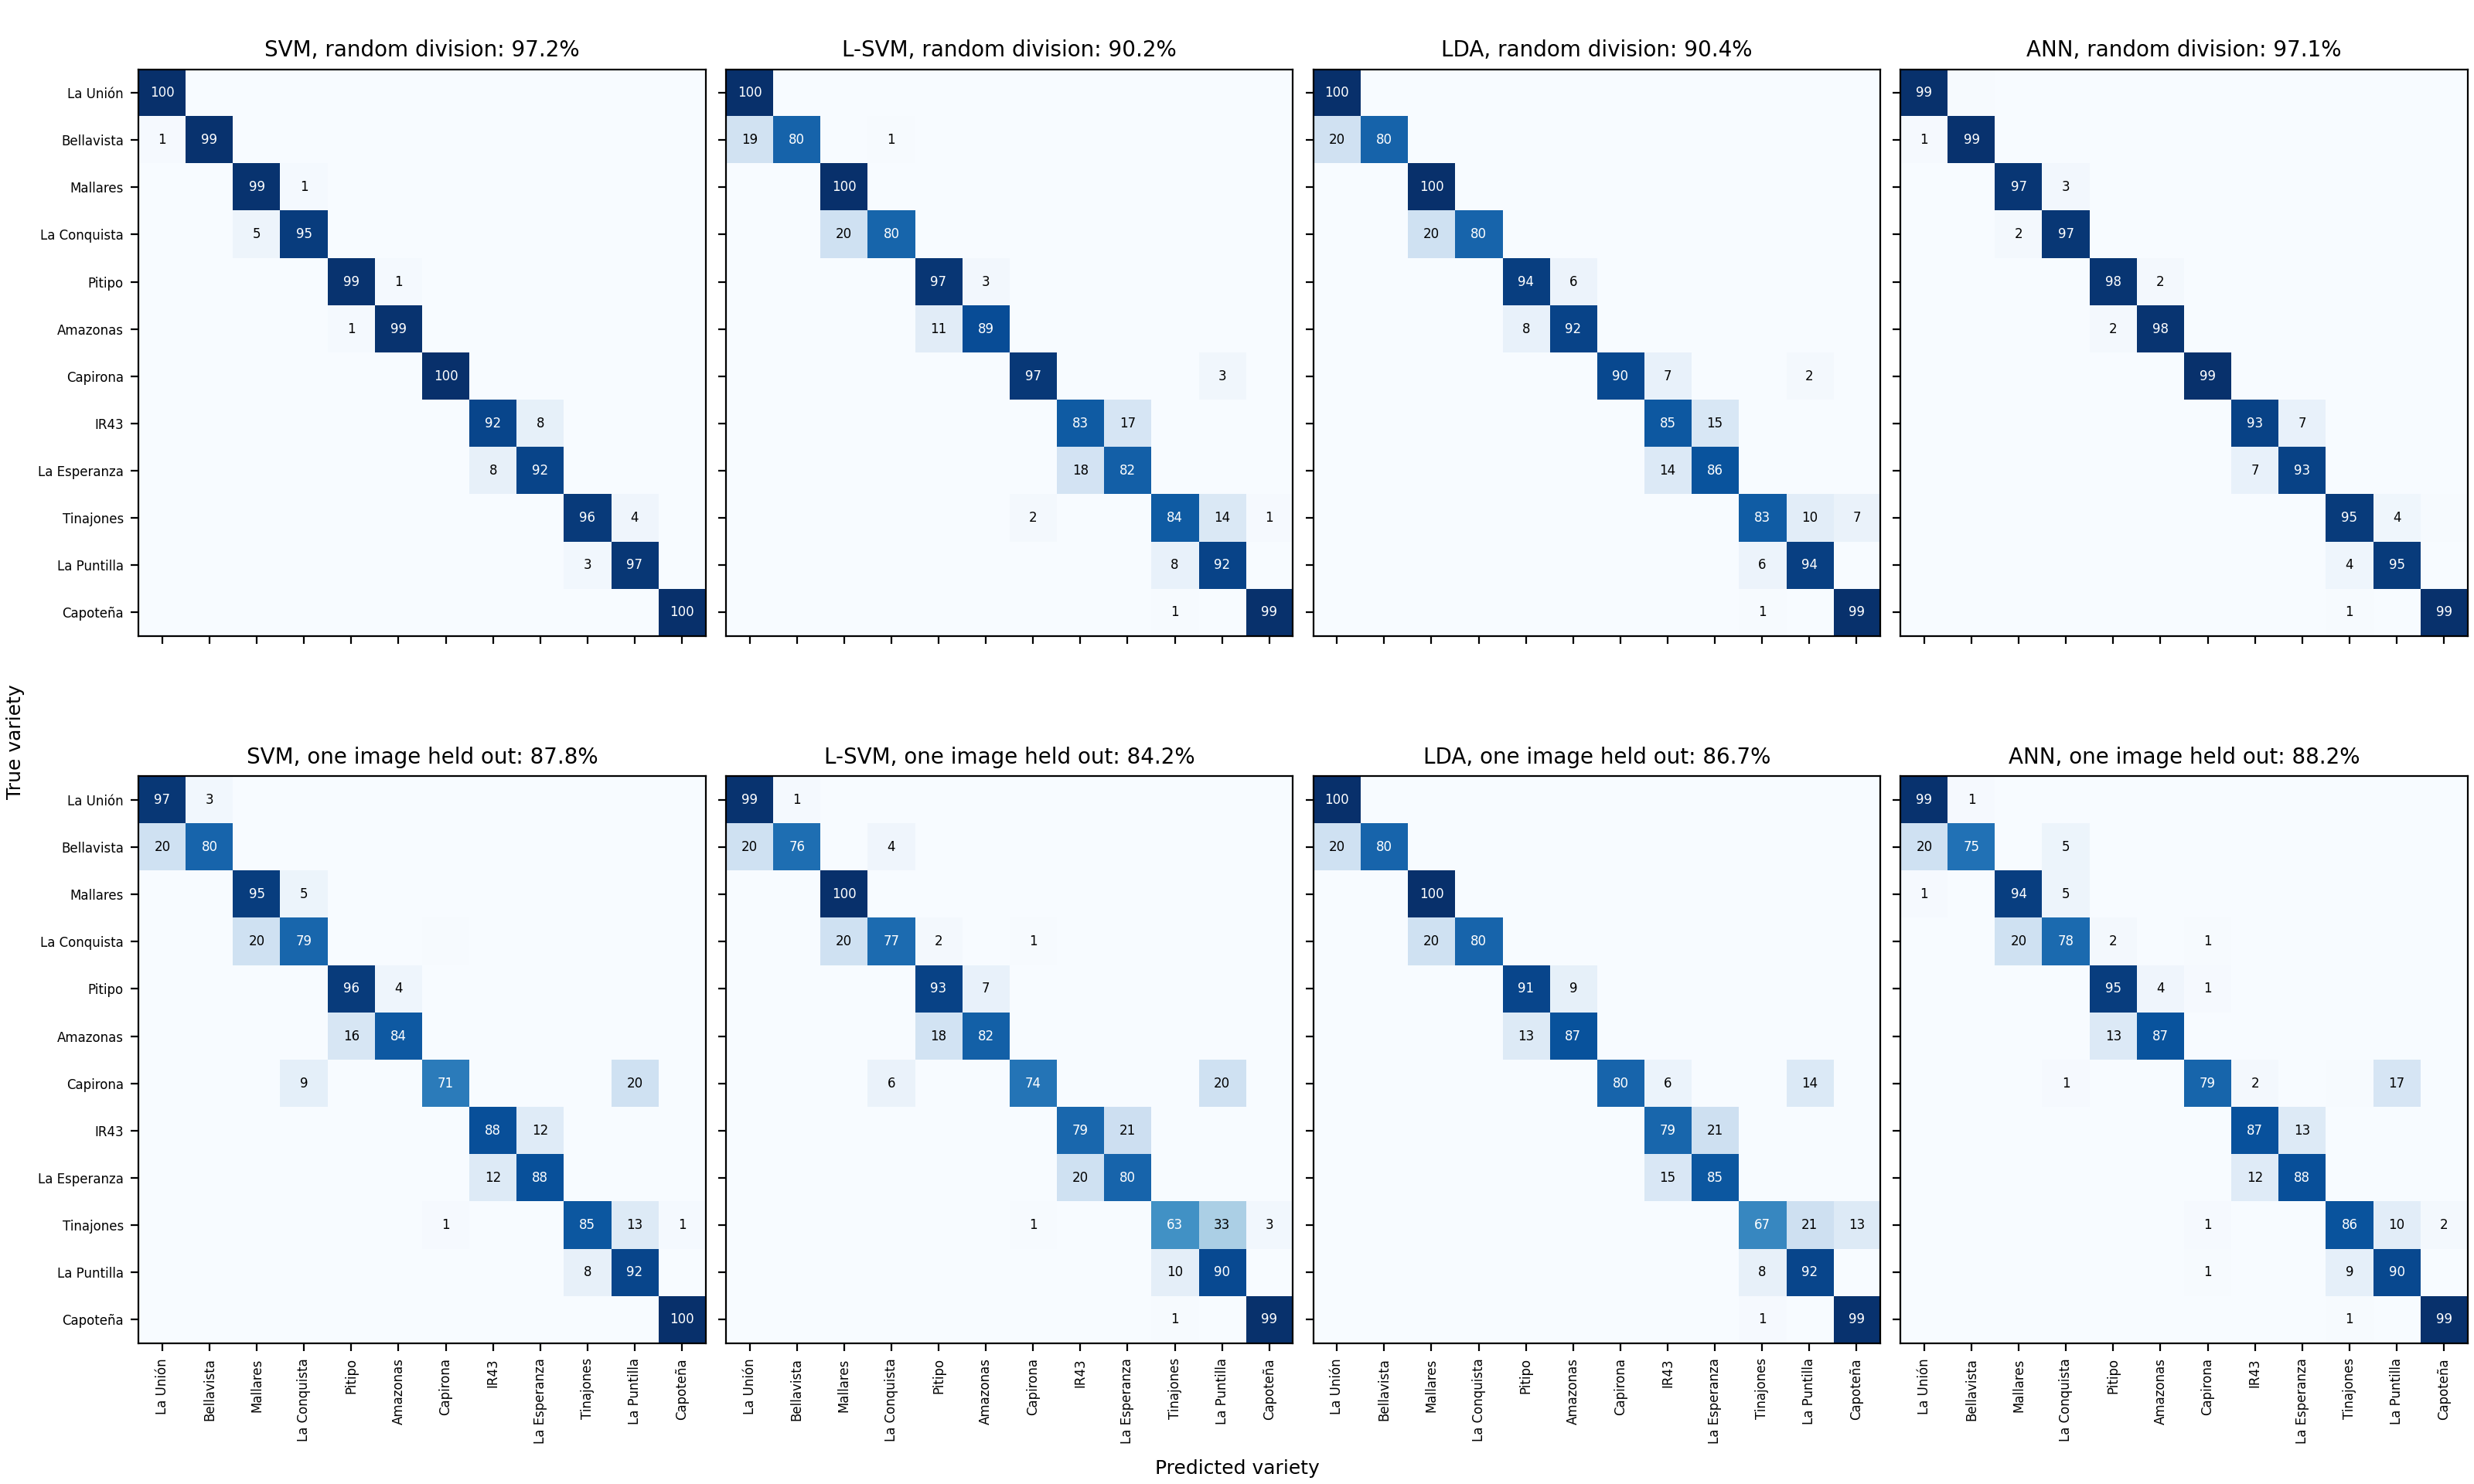
\includegraphics[width=\textwidth]{Figures/fig_unf_cm.png}
    \caption{\added{Confusion matrices (percent of the grains of each true variety, pooled over the 30 splits) of the four classifiers on the full spectrum: random division (top) and one image per variety held out (bottom). Panel titles give overall accuracy. Values below 0.5\% are not shown.}}
    \label{fig:cm}
\end{figure*}


\subsection{Random-subset baseline for band selection}\label{sec_bands_results}

\added{Each selection method was compared against randomly drawn band subsets of the same size, with one image per variety held out rather than under the random division, since an advantage from selecting bands only matters if it survives on grains from a new image. Each method was fitted on the training part of each of 10 splits (two repetitions of the grouped five-fold cross-validation, drawn independently of the 30 splits of Table~\ref{tab:acc}), with any internal cross-validation grouped in blocks of 10 rows; the subset it returned was evaluated on the test part with the SVM and the LDA classifier (the ANN and the L-SVM were left out to limit the cost: 1200 fits per classifier and method), and compared against 30 randomly drawn subsets of the same size on the same split. Because the internal cross-validation groups blocks of 10 rows rather than whole images, grains of one image can still sit on both sides of the internal criterion, which may reward bands specific to an acquisition. The three methods faced the same splits, and SFS and FSCNCA the same random subsets. SFS was implemented as forward selection with an LDA criterion scored by grouped five-fold cross-validation; feature-weighted NCA, the method behind MATLAB's \texttt{fscnca}, was implemented following \citet{Yang2012nca} and the bands ranked by their weights instead of thresholded; and CAFS was ported line by line from the MATLAB code. SFS (LDA criterion) and FSCNCA (bands ranked by their NCA weight) were evaluated at $k\in\{5,10,20,40\}$ bands. CAFS was run with the settings of the MATLAB v6 code (Section~\ref{sec_feature_selection}): SNV, naive Bayes scorer, a binary covering array of strength 2 and optimal size over the remaining bands (12 rows for 263 bands), and macro-F1 penalised for subsets larger than 20 bands. It sets its own subset size: the set shrinks from 263 to about 137, 80, 39, 24, 16 and 14 bands, and the algorithm returns the best-scoring subset over all iterations (7--25 bands). The subset of each iteration and the returned subset were compared against random subsets of the same size.}

\added{Tables~\ref{tab:bands_unf} and \ref{tab:bands_cafs} and Figure~\ref{fig:bands_unf} summarise the results. SFS beats the random mean at every $k$, by 6--9 points at $k=5$ and by at most 0.6 points at $k=40$. FSCNCA is never clearly better than random: 1.5--2.6 points ahead at $k\le10$, and level with or up to 1.4 points below random at $k=20$ and 40. CAFS falls 1.0--3.0 points below the random mean at every iteration shown, and the subset it returns -- 19 bands on average, from 7 to 25 depending on the split -- is also below random (80.1\% against 82.4\% with the SVM, 79.2\% against 82.2\% with LDA). In every case the selected subset falls inside the 5--95\% range of the random subsets. The advantage of selecting bands over drawing them at random is therefore at most modest, largest for SFS with very few bands, and vanishes as more bands are kept. Paired over the splits with Holm adjustment across the 30 comparisons, the paired $t$-test finds SFS better than random at 5 bands (by 6.2 points with the SVM and 8.8 with LDA; adjusted $p=0.002$ for both), at 10 bands (3.6 and 6.0 points; $p=0.007$ and $0.0007$) and at 20 bands with LDA only (2.3 points; $p=0.0005$); FSCNCA never better, and worse at 40 bands with the SVM (1.4 points, $p=0.010$); and CAFS never better, but worse than random at iterations 1--4 with the SVM (by 1.6--2.2 points, adjusted $p\le0.02$) and at iterations 2 and 3 with LDA (2.4 and 2.7 points, adjusted $p=0.042$ and $0.006$); its returned subset does not differ from random ($p=0.18$ with the SVM, $0.56$ with LDA). With 10 splits the Wilcoxon signed-rank test cannot reach an adjusted $p<0.05$ for any of the 30 comparisons (its smallest attainable unadjusted $p$ is 0.002), so these differences rest on the $t$-test alone, and the splits share images, so they are not independent.}
\added{The nine-band subsets obtained by applying each MATLAB routine once to all 6000 spectra (Figure~\ref{fig_04}) were tested directly against random nine-band subsets with one image per variety held out (Table~\ref{tab:sub9}). The SFS subset beats the random mean with all four classifiers, by 3.6--7.1 points, and outperforms 80--99\% of the random subsets; the FSCNCA subset beats it with the SVM, the L-SVM and LDA (2.4--4.2 points) but not with the ANN, whose hidden layer has only three units with nine bands; and the CAFS subset does not beat it with any classifier (and is 1.1 points below it with the L-SVM). These subsets were selected with all the spectra, so part of their advantage may come from the test grains taking part in the selection: when selection is fitted on the training part of each split, as above, FSCNCA no longer beats random subsets and SFS does so mainly with 5--10 bands.}

\begin{table*}[htbp!]
    \centering
    \caption{\added{Overall accuracy (\%, mean $\pm$ SD over the 30 splits, one image per variety held out) of the nine-band subsets obtained by applying each MATLAB routine once to all the spectra, against 30 random nine-band subsets per split (mean, and 5--95\% range over all random draws). Fraction: share of random subsets outperformed, averaged over splits. The subsets were selected with all the spectra, which favours them. With nine bands the ANN has three hidden units.}}
    \label{tab:sub9}
    \begin{tabular}{llcccc}
    \hline
    Classifier & Subset & Accuracy & Random mean (5--95\%) & Difference & Fraction \\
    \hline
    SVM   & FSCNCA & 83.2 $\pm$ 7.3 & 80.8 (69.1--91.8) & $+$2.4 & 0.74 \\
          & SFS    & 84.3 $\pm$ 7.0 & 80.8 (69.1--91.8) & $+$3.6 & 0.88 \\
          & CAFS   & 79.8 $\pm$ 6.8 & 80.8 (69.1--91.8) & $-$0.9 & 0.35 \\
    L-SVM & FSCNCA & 73.3 $\pm$ 7.2 & 69.1 (55.0--80.2) & $+$4.2 & 0.81 \\
          & SFS    & 76.2 $\pm$ 6.9 & 69.1 (55.0--80.2) & $+$7.0 & 0.99 \\
          & CAFS   & 68.0 $\pm$ 5.8 & 69.1 (55.0--80.2) & $-$1.1 & 0.34 \\
    LDA   & FSCNCA & 81.7 $\pm$ 7.3 & 78.7 (65.8--90.5) & $+$3.0 & 0.79 \\
          & SFS    & 85.2 $\pm$ 7.0 & 78.7 (65.8--90.5) & $+$6.5 & 0.97 \\
          & CAFS   & 79.3 $\pm$ 7.2 & 78.7 (65.8--90.5) & $+$0.6 & 0.54 \\
    ANN   & FSCNCA & 72.5 $\pm$ 11.1 & 71.1 (56.2--83.8) & $+$1.4 & 0.56 \\
          & SFS    & 78.3 $\pm$ 7.1 & 71.1 (56.2--83.8) & $+$7.1 & 0.80 \\
          & CAFS   & 71.7 $\pm$ 5.2 & 71.1 (56.2--83.8) & $+$0.5 & 0.50 \\
    \hline
    \end{tabular}
\end{table*}
\acnote{Computed on GUANE with our scripts \texttt{19\_Subconjuntos\_UNF.py} and \texttt{20\_Inferencia\_imagen.py}; results in \texttt{resultados\_UNF\_v4\_inferencia.xlsx}. Holm-adjusted over 12 comparisons: SFS and FSCNCA (except FSCNCA with the ANN) above random at $p<10^{-4}$; CAFS not above random (with the L-SVM below it, $p=0.002$).}

\acnote{Significance tests computed with our script \texttt{12\_Significancia.py} (Python, SciPy) on the per-split results of \texttt{10\_Validacion\_UNF.py} and \texttt{14\_CAFS\_v6\_baseline.py}, run on the GUANE cluster; full tables in \texttt{resultados\_UNF\_significancia.xlsx}. CAFS iterations reached by fewer than 9 of the 10 splits were excluded from the tests and from Table~\ref{tab:bands_cafs}.}


\begin{table*}[htbp!]
    \centering
    \caption{\added{Overall accuracy (\%, mean $\pm$ SD) of SFS- and FSCNCA-selected bands against 30 randomly drawn subsets of the same size, with one image per variety held out (10 splits; same splits and random subsets for both methods). The SD of the random subsets is over 300 evaluations (30 subsets in each of 10 splits), that of SFS and FSCNCA over the 10 splits.}}
    \label{tab:bands_unf}
    \resizebox{0.75\textwidth}{!}{
    \begin{tabular}{rcccccc}
    \hline
    \multirow{2}{*}{Bands $k$} & \multicolumn{3}{c}{SVM} & \multicolumn{3}{c}{LDA} \\
     & SFS & FSCNCA & Random & SFS & FSCNCA & Random \\
    \hline
    5  & 80.2 $\pm$ 5.6 & 76.1 $\pm$ 6.8 & 74.0 $\pm$ 7.4 & 79.8 $\pm$ 3.9 & 73.6 $\pm$ 7.7 & 71.0 $\pm$ 6.3 \\
    10 & 84.2 $\pm$ 6.7 & 82.1 $\pm$ 5.6 & 80.6 $\pm$ 6.7 & 85.0 $\pm$ 4.4 & 81.4 $\pm$ 4.2 & 79.0 $\pm$ 5.2 \\
    20 & 85.5 $\pm$ 5.8 & 83.1 $\pm$ 6.0 & 83.6 $\pm$ 6.2 & 86.2 $\pm$ 4.2 & 84.2 $\pm$ 4.8 & 83.8 $\pm$ 4.5 \\
    40 & 85.3 $\pm$ 6.3 & 83.9 $\pm$ 6.4 & 85.3 $\pm$ 6.1 & 86.5 $\pm$ 4.5 & 85.4 $\pm$ 5.2 & 85.9 $\pm$ 4.8 \\
    \hline
    \end{tabular}
    }
    
    
\end{table*}

\begin{table*}[htbp!]
    \centering
    \caption{\added{Overall accuracy (\%, mean $\pm$ SD over splits) of CAFS-selected bands against 30 randomly drawn subsets of the same size, with one image per variety held out (10 splits). CAFS (settings of the MATLAB v6 code) sets its own subset size, so sizes are means over the splits that reached each iteration; iterations 7--9, reached by 5, 2 and 1 of the 10 splits, are not shown. Last row: the subset CAFS returns, the best-scoring over all iterations.}}
    \label{tab:bands_cafs}
    \begin{tabular}{rccccc}
    \hline
    \multirow{2}{*}{Bands (mean)} & \multirow{2}{*}{Splits} & \multicolumn{2}{c}{SVM} & \multicolumn{2}{c}{LDA} \\
     & & CAFS & Random & CAFS & Random \\
    \hline
    137 & 10 & 85.0 $\pm$ 6.5 & 86.7 $\pm$ 6.2 & 85.5 $\pm$ 5.6 & 86.5 $\pm$ 4.9 \\
    80  & 10 & 84.1 $\pm$ 6.8 & 86.2 $\pm$ 6.1 & 84.1 $\pm$ 5.4 & 86.5 $\pm$ 4.8 \\
    39  & 10 & 83.3 $\pm$ 6.5 & 85.2 $\pm$ 6.1 & 83.2 $\pm$ 5.1 & 85.9 $\pm$ 4.6 \\
    24  & 10 & 81.9 $\pm$ 6.5 & 84.1 $\pm$ 6.0 & 82.0 $\pm$ 5.8 & 84.6 $\pm$ 4.5 \\
    16  & 10 & 79.4 $\pm$ 6.8 & 82.4 $\pm$ 5.8 & 79.9 $\pm$ 7.0 & 82.4 $\pm$ 4.7 \\
    14  & 10 & 78.4 $\pm$ 6.3 & 80.9 $\pm$ 5.7 & 78.0 $\pm$ 6.1 & 80.4 $\pm$ 5.7 \\
    \hline
    Returned, 19 (7--25) & 10 & 80.1 $\pm$ 6.6 & 82.4 $\pm$ 5.7 & 79.2 $\pm$ 5.8 & 82.2 $\pm$ 5.2 \\
    \hline
    \end{tabular}
\end{table*}

\begin{figure*}[htbp!]
    \centering
    \subfloat[SFS]{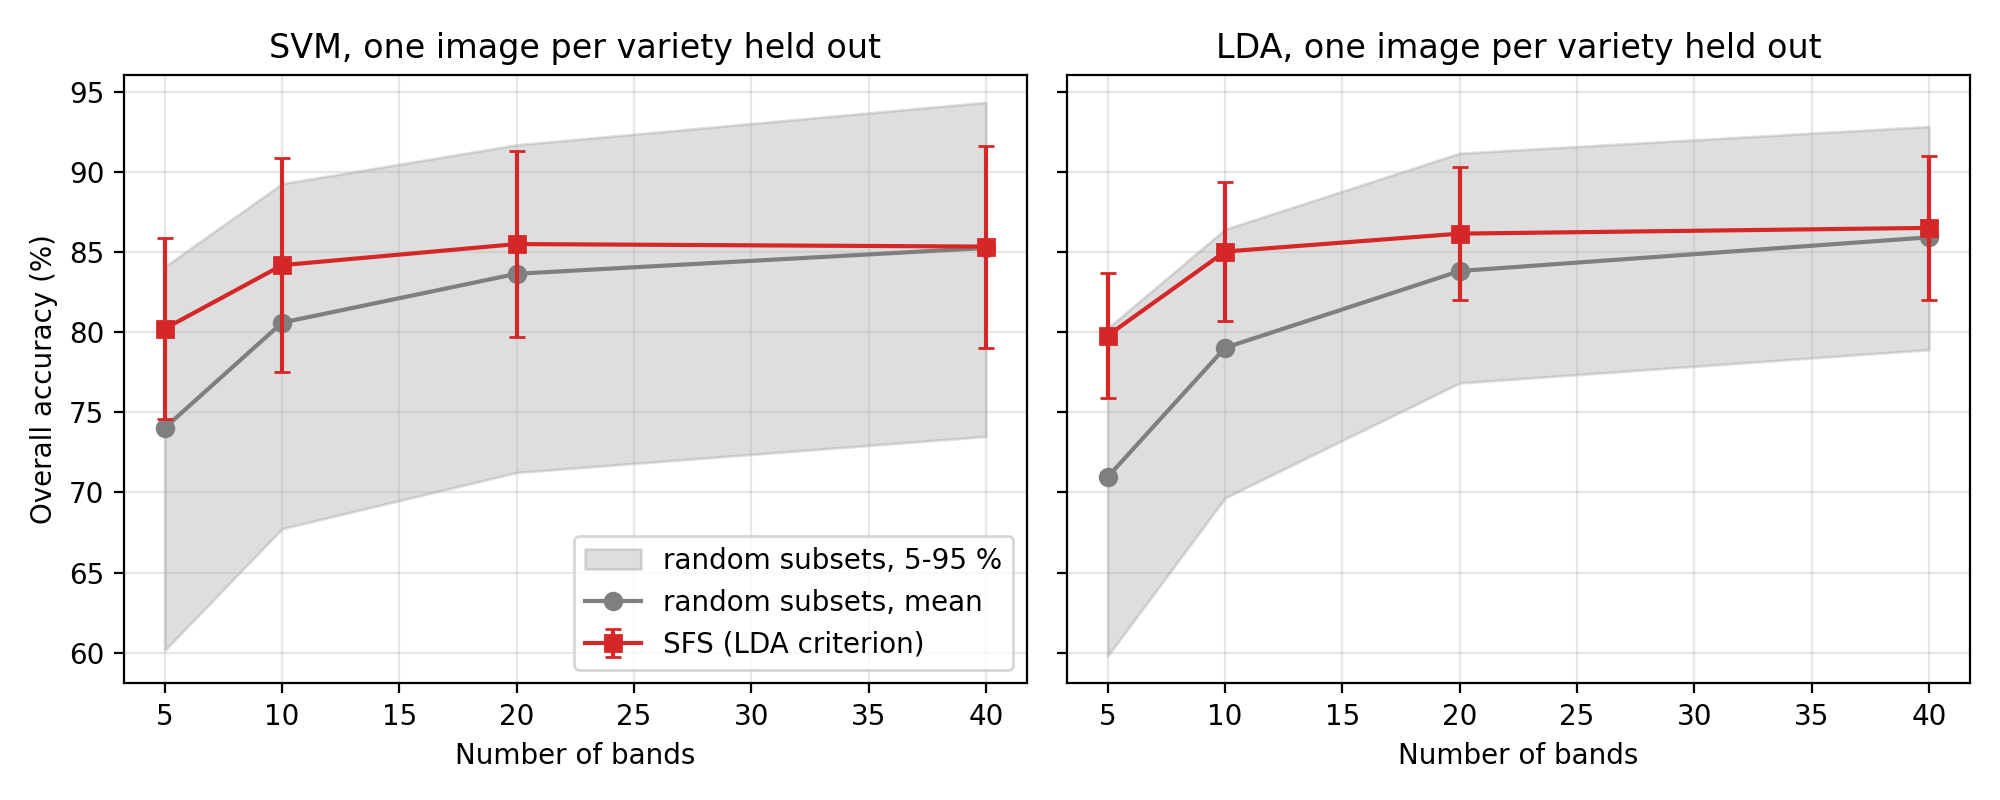
\includegraphics[width=0.49\textwidth]{Figures/fig_unf_bandas.png}}
    \hfill
    \subfloat[FSCNCA]{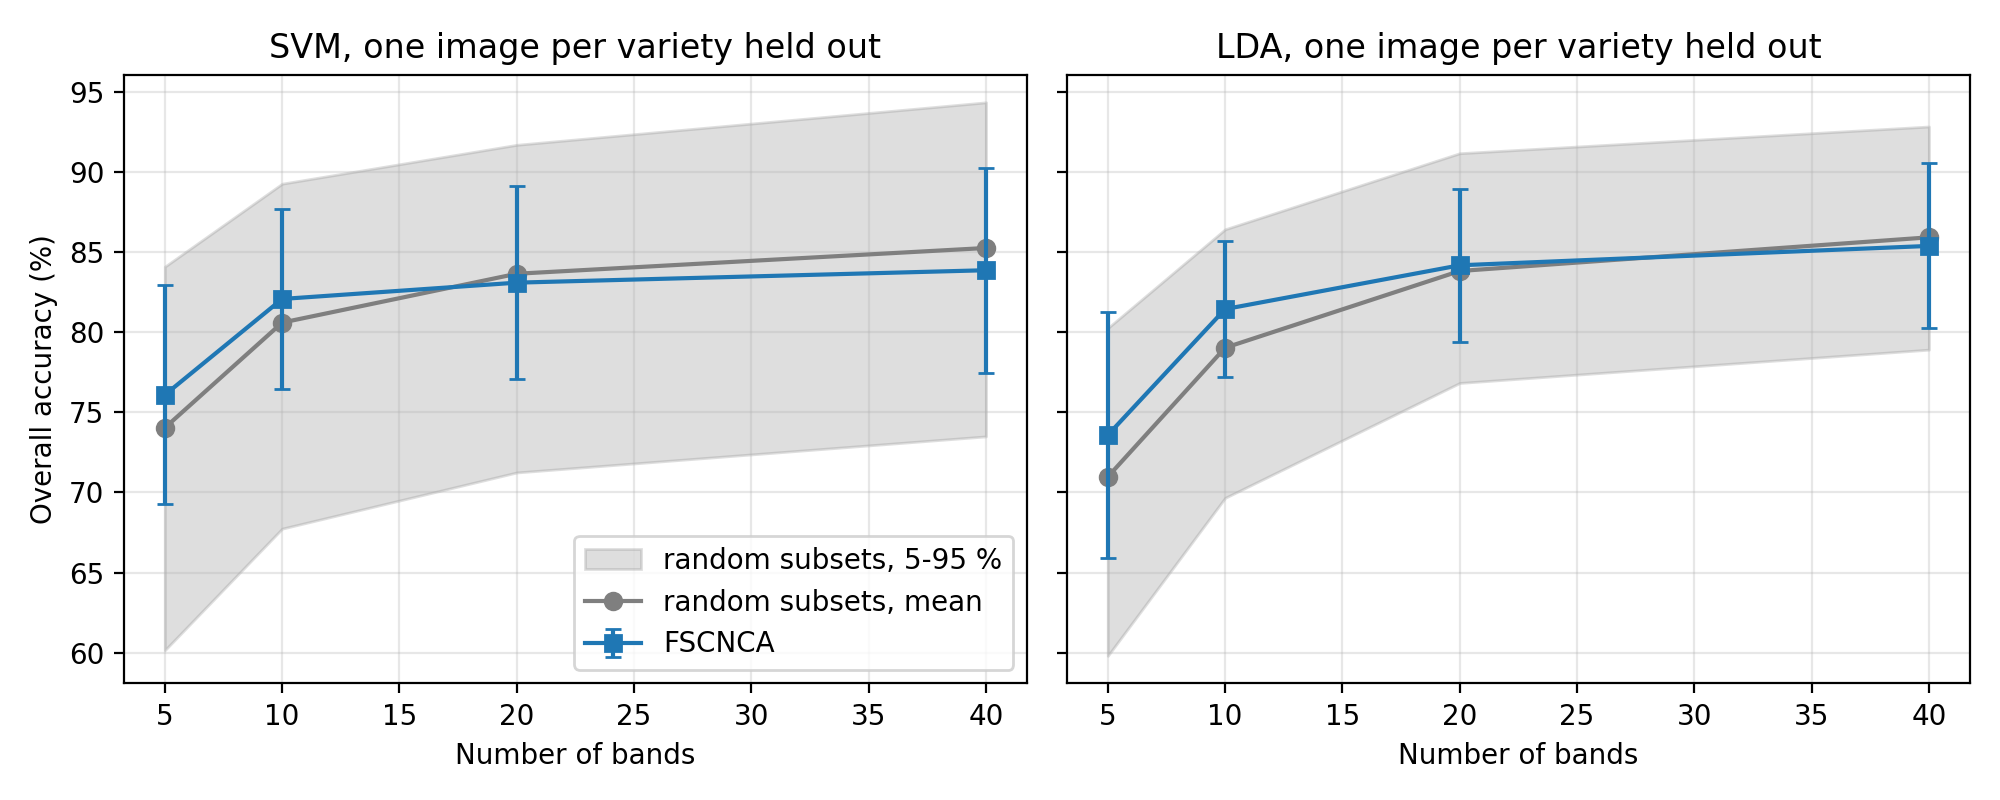
\includegraphics[width=0.49\textwidth]{Figures/fig_unf_bandas_fscnca.png}}\\
    \subfloat[CAFS]{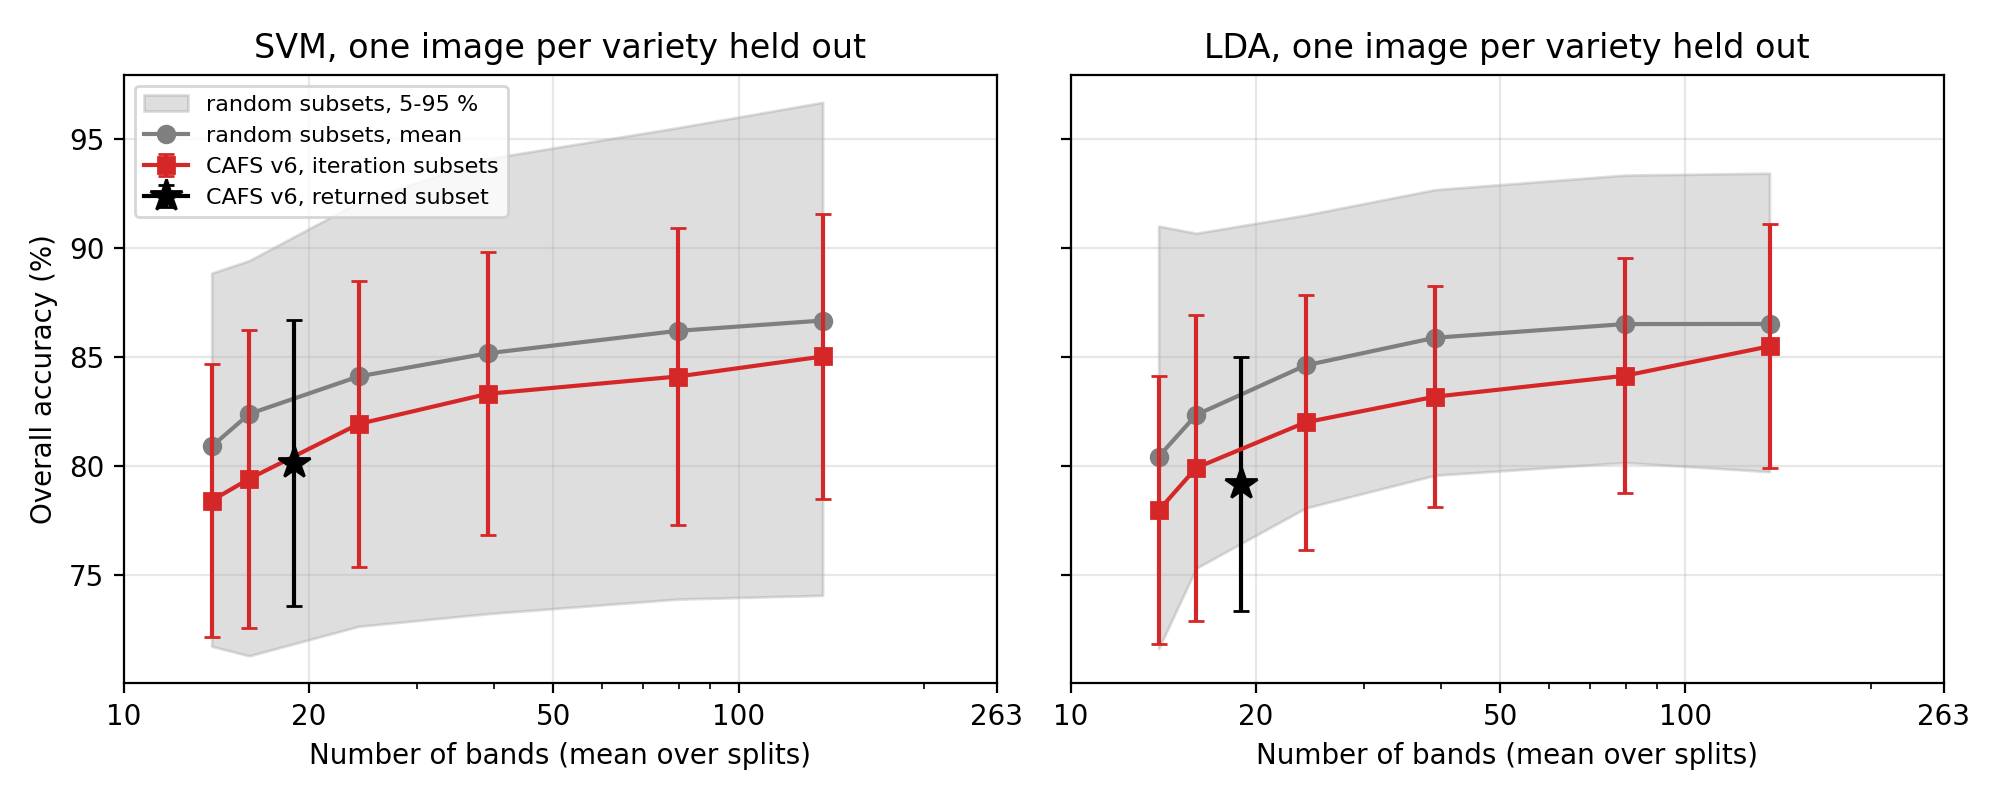
\includegraphics[width=0.49\textwidth]{Figures/fig_unf_bandas_cafs_v6.png}}
    \caption{Overall accuracy of band subsets selected by (a) SFS, (b) FSCNCA and (c) CAFS (coloured), against 30 randomly drawn subsets of the same size (grey mean and 5--95\% band), with one image per variety held out, for SVM (left) and LDA (right). In (c) the horizontal axis is logarithmic and gives the mean subset size per CAFS iteration (iterations reached by at least 9 of the 10 splits); the star is the subset CAFS returns.}
    \label{fig:bands_unf}
\end{figure*}

\acnote{How these three baselines were computed, so that you can check them against your MATLAB code (all in Python 3.14, scikit-learn 1.9, scripts in our \texttt{draft\_UNF\_conjunto} folder). \textbf{SFS}: our own implementation in \texttt{10\_Validacion\_UNF.py}, forward selection with an LDA criterion scored by grouped 5-fold CV. \textbf{FSCNCA}: MATLAB's \texttt{fscnca} has no Python equivalent, so we wrote feature-weighted NCA following Yang, Wang and Zuo (2012), also in \texttt{10\_Validacion\_UNF.py}: L1 distance with squared weights, kernel width $\sigma=1$, $\lambda=1/n$, weights initialised at 1, optimised with Adam (learning rate 0.02, 150 iterations) on a subsample of 100 training rows per variety; bands ranked by weight. Your threshold sweep (1--6 in steps of 0.5; fixed at 3.6 in the reported run) was replaced by taking the top $k$. \textbf{CAFS}: a line-by-line port of your \texttt{cafs\_matlab\_classification\_v6.m} (functions \texttt{cafs\_inner\_selection\_v2}, \texttt{compute\_selection\_score}, \texttt{generate\_CA\_2\_k\_2}) in \texttt{14\_CAFS\_v6\_baseline.py}, with the options of \texttt{b\_AnalizarPerfilesArroz\_2.m}: SNV, Gaussian naive Bayes, Patience = 3, MinImprovement = $10^{-4}$, MinFeatures = 10, MaxIterations = 50, TargetFeatures = 20, CompactnessPenalty = 0.10, ExcessPenaltyPower = 2, AdaptivePenaltyAlpha = 2. Our covering-array generator reproduces your \texttt{coveringArray\_last\_generated.csv} exactly. Two differences: the inner 5-fold cross-validation is stratified and grouped over blocks of 10 rows (StratifiedGroupKFold) rather than \texttt{cvpartition}, so that selection does not use grains of the same acquisition block for fitting and scoring, as in the other baselines; and there is no hyperparameter search for a final naive Bayes model, because each subset is evaluated with the SVM and LDA. An earlier baseline built from the PyPI package \texttt{cafspy} 0.0.1 (\texttt{11\_CAFS\_baseline.py}, before we had your code) is superseded and kept only in our records.}



\added{\section{Discussion}\label{sec_discussion}

\subsection{Validation design and metric}
The accuracies obtained under random and grouped division estimate different quantities. Under the random division the test grains come from images also represented in training; with an image held out they come from another image of the same lot, which is closer to how an instrument would be used, though still optimistic for a new lot, season or session. The gap between them, about 9 points for the SVM, depends on how much grains imaged together share, a property of the acquisition rather than of the classifier, so it cannot be carried to another data set as a correction. The same distinction bears on the choice of classifier: the 7-point lead of the SVM and the ANN over LDA and the L-SVM under the random division disappears against LDA with an image held out, where the SVM, the ANN and LDA no longer differ, and shrinks to 3.7 points against the L-SVM. The per-class one-vs-rest accuracy, in turn, compresses differences by a factor of six for twelve classes and cannot fall below 83.3\%. The studies in Table~\ref{Table1} report accuracies of 90--100\%; where a study does not state whether grains from one image or session were kept together, or which accuracy it reports, its figures and ours cannot be compared as they stand.

\subsection{Band selection}
The three selection methods retained different bands (Figure~\ref{fig_04}). The original nine-band subsets beat random nine-band subsets for SFS and largely for FSCNCA, but not for CAFS (Table~\ref{tab:sub9}); because they were chosen with all the spectra, the training-only analysis is the fairer test. Fitted on training data only and tested on held-out images, SFS beat randomly drawn subsets of the same size at 5 and 10 bands, by 4--9 points -- the range that matters for an instrument with few channels -- and at 20 bands with LDA, but not at 40; FSCNCA led random subsets by at most 2.6 points and not at all from twenty bands on; and CAFS trailed them by 1.0--3.0 points at every size. Neighbouring NIR bands are highly correlated, so a well-spread subset of adequate size retains most of what a ranked subset does. A band-selection result on spectra of this kind should therefore be reported against a random-subset control of the same size.

\subsection{Chemical interpretation}
The features that differ most between the mean profiles are the C--H second-overtone absorption near 1200~nm, shared by starch and lipid, and the O--H absorption of water above about 1400~nm (Section~\ref{sec_mean_profiles}). These differences are consistent with differences in starch structure, lipid and moisture between varieties, but this paper does not test that attribution, which would require composition measured on the same grains that were imaged.

\subsection{Limitations}\label{sec_limitations}
Each variety is a single lot imaged in one session, so variety is confounded with lot and acquisition time. The confused pairs have consecutive codes, which suggests that the varieties were imaged in that order and that slow changes in the instrument contribute to the similarity of neighbouring varieties. Three of the 60 images -- image~5 of Bellavista, image~1 of La Conquista and image~5 of Capirona -- are classified almost entirely as La Uni\'on, Mallares and La Puntilla when held out, which points to a labelling or sample slip that only the acquisition records can confirm; they are kept here with their labels as received. They are the extreme cases of a wider image effect: three more images (image~1 of Amazonas, image~1 of La Esperanza and image~3 of Tinajones) have fewer than two thirds of their grains classified correctly by every classifier. Finally, the grouping into images of 100 grains follows the acquisition protocol and has not been checked against image identifiers.}
\acnote{Please check the three images (consecutive blocks of 100 rows per variety in the shared matrix) and confirm that the 500 rows of each variety are five images of 100 grains in acquisition order.}

\section{Conclusion}

\added{Twelve Peruvian rice varieties can be distinguished from NIR-HSI spectra of single grains, with an overall accuracy of about 97\% for the linear SVM and the ANN when grains are divided at random and about 88\% when whole images are held out; LDA reaches 90\% and 87\%, and the L-SVM 90\% and 84\%. Reporting the per-class one-vs-rest accuracy instead would show 99.5\% and hide most of this difference. With images held out, the SVM, the ANN and LDA do not differ. Band selection reduced the number of bands without consistently identifying better ones: fitted on training data only, only SFS beat randomly drawn subsets of the same size, and only with few bands; nine-band subsets selected once with all the spectra did better for SFS and FSCNCA, but the test grains took part in choosing them. Reporting overall accuracy, validating on images not used for training, and benchmarking band selection against random subsets would make accuracies comparable across studies.}



% ================================================================================================
\added{\section*{Declaration of generative AI and AI-assisted technologies}
During the preparation of this work the authors used Claude Code (Anthropic, Claude Opus 5.5 model) to write and run the analysis code and statistics and to draft parts of the text. The authors reviewed and edited all content, verified every reported result and reference, and take full responsibility for the content of the published article. Code and a dated record of the analysis are available [PENDING: repository or ``from the corresponding author''].}
\acnote{Elsevier requires this declaration. It describes how the revision was done at UNISUCRE; please check that it also covers the original MATLAB analysis (if any AI tool was used there, add it) and tell us whether you agree to publishing the code in a public repository.}

%% BIBLIOGRAPHY
% ================================================================================================
\bibliographystyle{elsarticle-num-names}
\bibliography{references2}

\end{document}
